% {{{ Packages

% {{{ Versions
% version écran
\documentclass{beamer}

% version orateur
%\setbeameroption{show only notes}
%\usepackage{pgfpages}
%\pgfpagesuselayout{2 on 1}[a4paper,border shrink=5mm]

% version spectateur
%\documentclass[handout]{beamer}
%\usepackage{handoutWithNotes}
%\pgfpagesuselayout{1 on 1 with notes}[a4paper,border shrink=5mm]
% }}}

\usepackage[utf8]{inputenc}
\usepackage[french]{babel}
\usepackage{tikz}
\usepackage{caption}
\usetheme{Goettingen}

% }}}
% {{{ Commands
\makeatletter
\def\ft@overlay{}

\addtobeamertemplate{footline}{}
{
    \lineskiplimit0pt
    \begin{tikzpicture}[remember picture,overlay]
        \ft@overlay
    \end{tikzpicture}
    \gdef\ft@overlay{}
}

\newcommand<>{\addtooverlay}[1]{
    \only#2{
      \expandafter\gdef\expandafter\ft@overlay\expandafter{\ft@overlay
          \draw[fill=black,opacity=0.70]
              (current page.north east) rectangle (current page.south west);
          \node[text=white] at (current page.center) {
              #1
          };
      }
    }
    \pause
}
% }}}

\title{Pushing (a little) the limits \\
    of your DIY electronics}
\author{Sanpi}
\date{30 juin 2016}

\begin{document}
% {{{ Titre
\begin{frame}
    \titlepage
\end{frame}
% }}}

% {{{ Introduction
\section{Introduction}
\begin{frame}
    \frametitle{Introduction}

    \addtooverlay<.(1)>{
        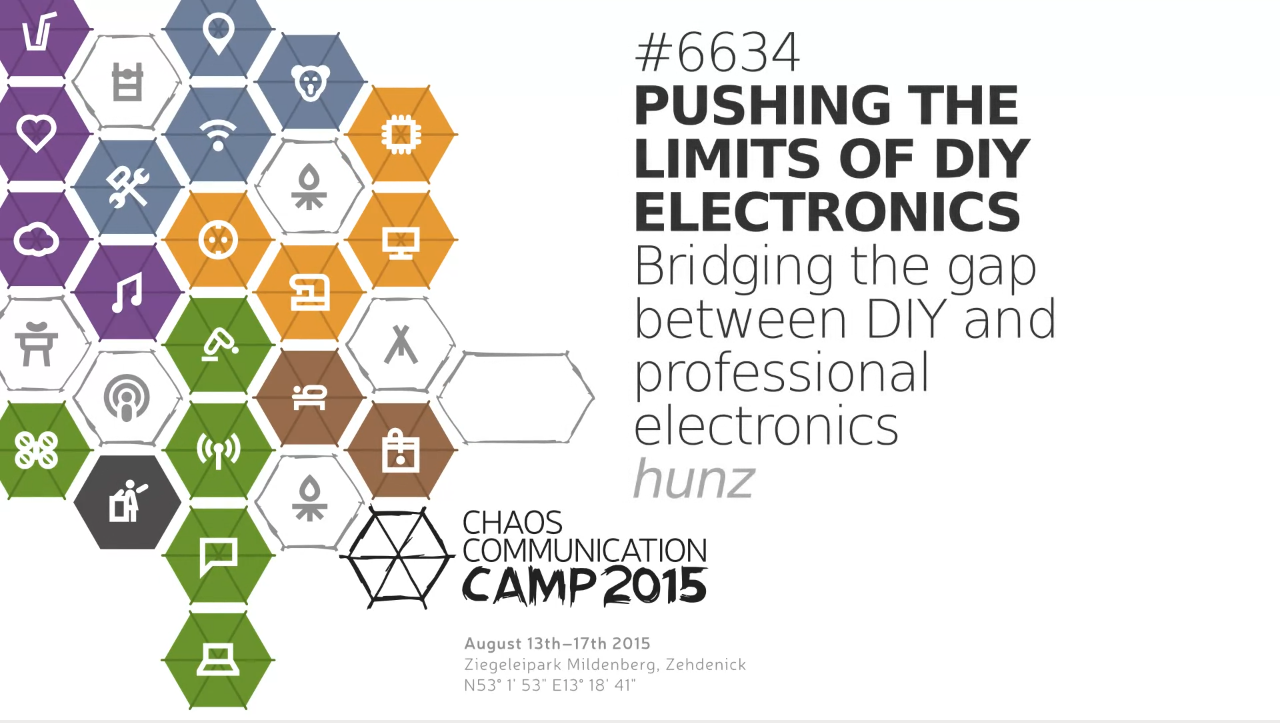
\includegraphics[scale=0.25]{images/ccc}
    }
    \addtooverlay<.(1)>{
        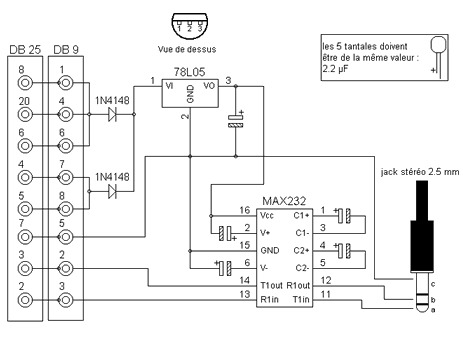
\includegraphics[scale=0.28]{images/cable-casio-pc}
    }
    \addtooverlay<.(1)>{
        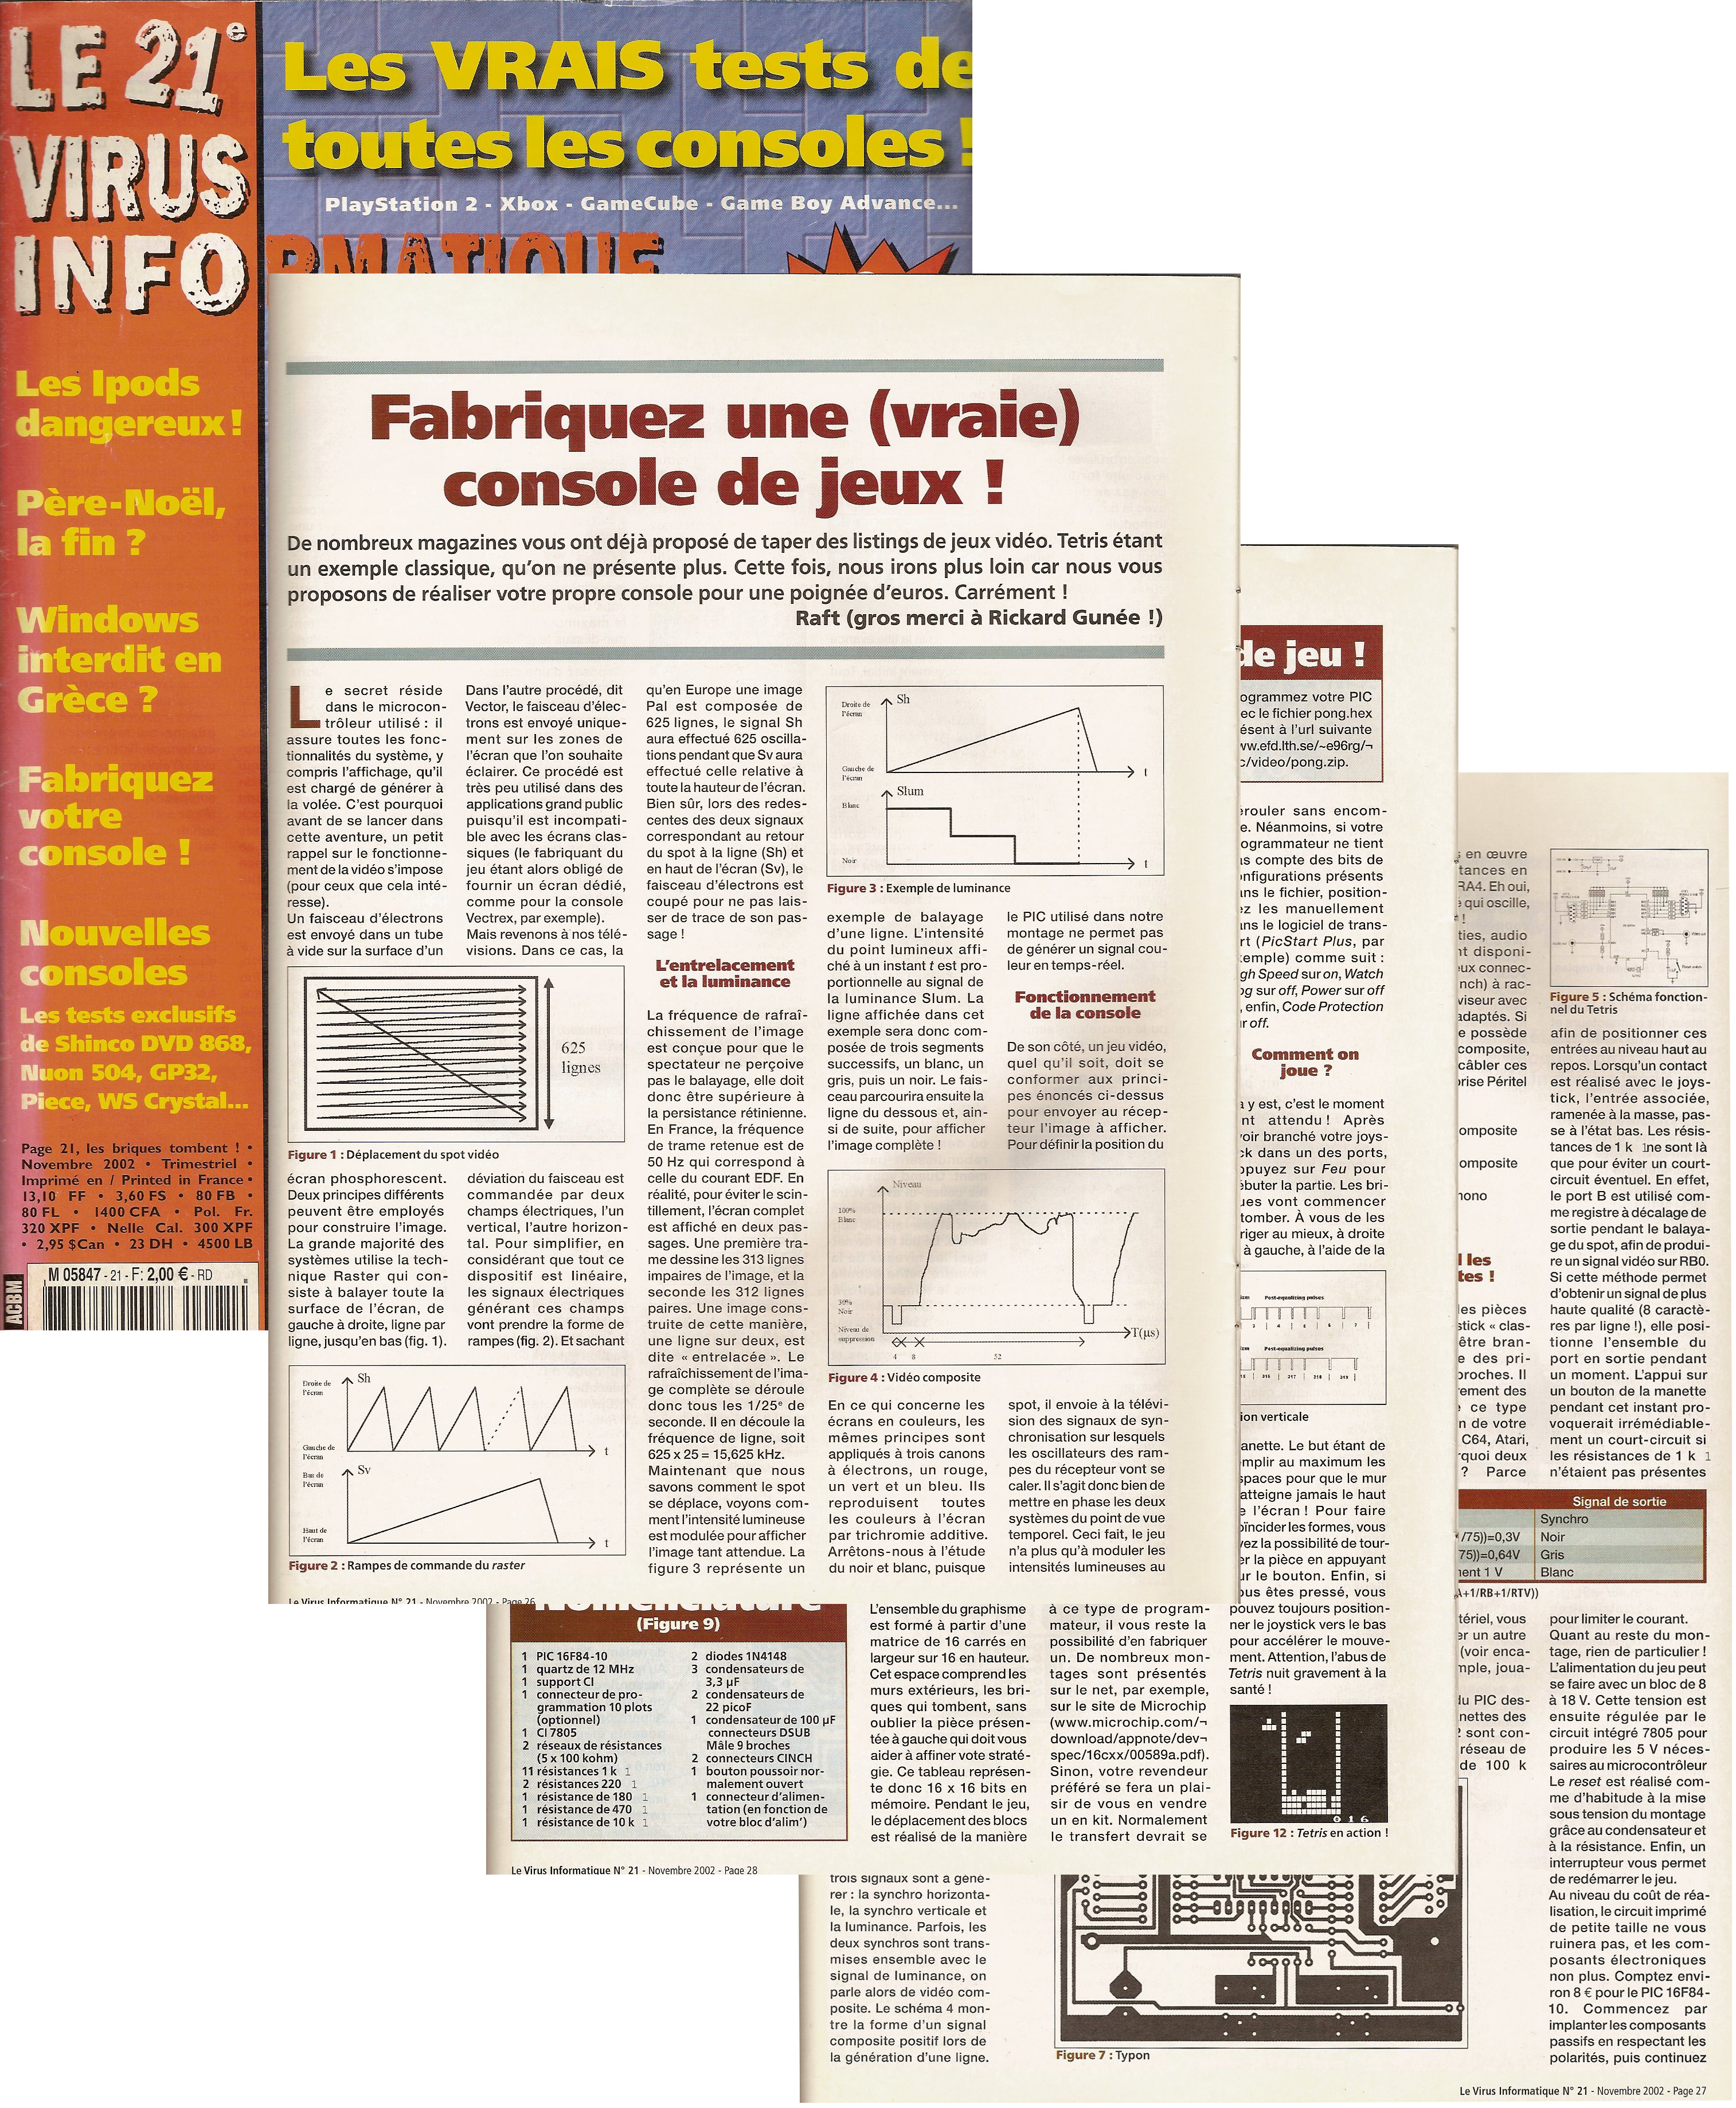
\includegraphics[scale=0.20]{images/virus}
    }
\end{frame}

\note[itemize] {
    \item Le titre une référence à la conférence donnée lors du CCC, l’année
        dernière.  Conférence à laquel j’ai assisté pensant, que j’allais
        comprendre quelque chose. Donc l’idée de cette présentation est d’aller
        un peu plus loin dans l’électronique amateur tout en restant simple.
        Pour vous donner une idée mon niveau dans ce domaine, autant que je m’en
        souvienne, j’ai fait de l’électronique au collège et ensuite peux de
        chose.

    \item J’ai soudé un cable pour calculatrice casio, pour m’éviter le recopie
        pénible de jeux en basic, qui fonctionnait très bien.

    \item Ensuite j’ai essayé de faire une console publiée dans un magazine, qui
        n’a pas fonctionné.

    \item Et c’est tout.
}
% }}}

% {{{ Arduino
\section{Arduino}
\begin{frame}
    \tableofcontents[currentsection]
\end{frame}

\note[itemize] {
    \item Jusqu’à ce que je découvre avec l’arduino en 2010. Ça m’a permit de
        redécouvrir que l’électronique ce n’est pas très compliqué.
}
% {{{ L’IDE
\begin{frame}
    \frametitle{L’IDE}

    \addtooverlay<.(1)>{
        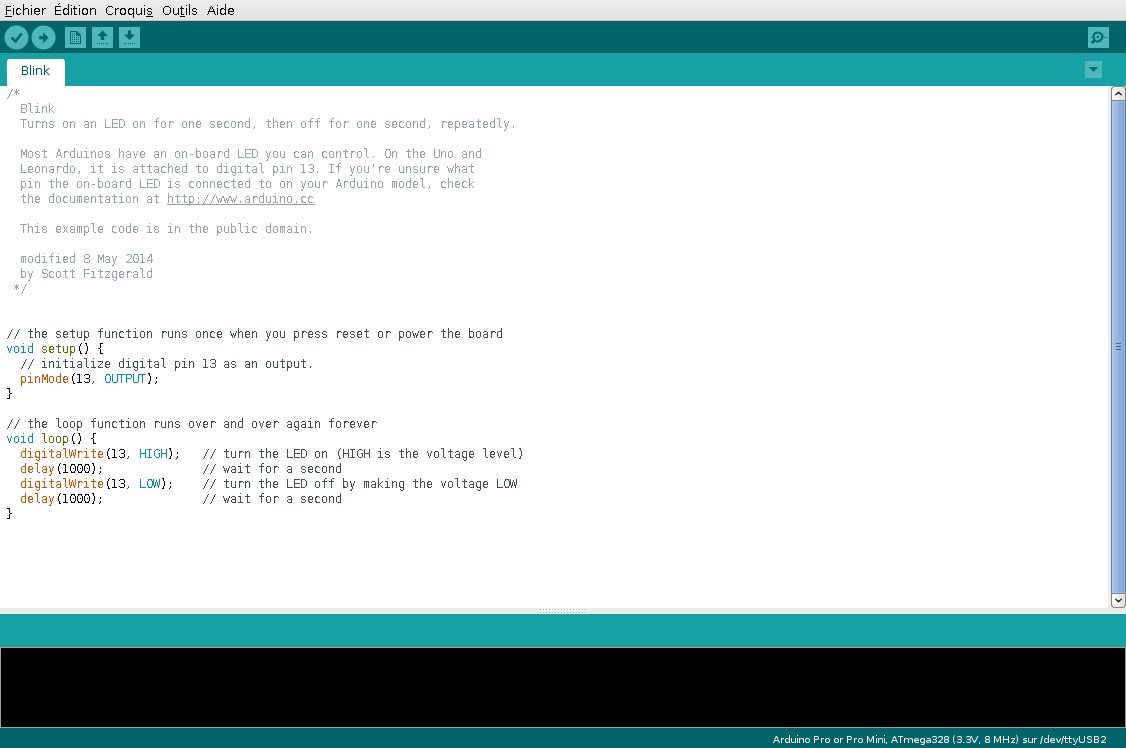
\includegraphics[scale=0.28]{images/arduino/ide}
    }
    \addtooverlay<.(1)>{
        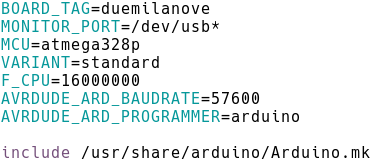
\includegraphics[scale=0.4]{images/sources/makefile}
    }
    \addtooverlay<.(1)>{
        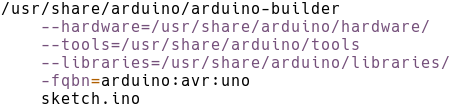
\includegraphics[scale=0.4]{images/sources/builder}
    }
\end{frame}

\note[itemize] {
    \item La première chose qui m’a agacée c’est l’IDE. En tant qu’utilisateur
        de vim, j’ai beaucoup de mal à utiliser un autre éditeur de texte.

    \item Jusqu’à la version 1.5, c’était simple il sufisait d’inclure un
        template dans votre makefile pour retrouver un bon vieux `make` puis
        `make upload`.

    \item Malheureusement, depuis la dernière version, le `Makefile.mk` à
        disparu. À la place nous avons un outils `arduino-builder` qui manque de
        documentation mais qui fait le travail. Il suffit de ceci dans un
        makefile et on retombe sur nos pieds.

    \item Bon, une fois l’IDE remplacé, on se rend compte que l’on embarque
        beaucoup de chose pour faire clignoter une led. Attaquons nous à la
        partie logicielle.
}
% }}}
% {{{ Le logiciel
\begin{frame}
    \frametitle{Le logiciel}
\end{frame}

\begin{frame}
    \frametitle{Le logiciel}

    \addtooverlay<.(1)>{
        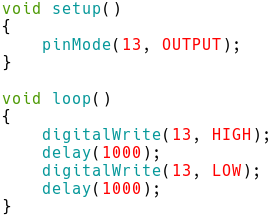
\includegraphics[scale=0.4]{images/sources/ino}
    }
    \addtooverlay<.(1)>{
        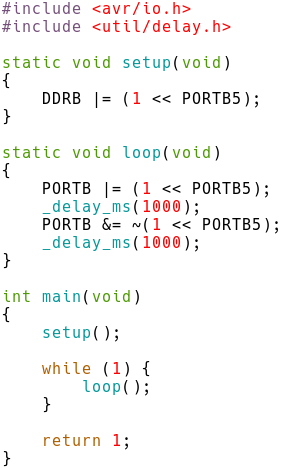
\includegraphics[scale=0.4]{images/sources/c}
    }
    \addtooverlay<.(1)>{
        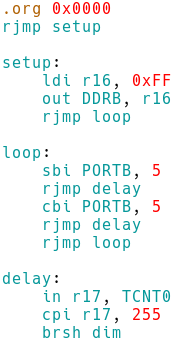
\includegraphics[scale=0.4]{images/sources/asm}
    }
\end{frame}

\note[itemize] {
    \item La bibliothèque arduino est conçue pour supportée toutes la gamme de
        carte ardiuno ce qui alourdi grandement le binaire produit. Par exemple,
        pour faire clignoter une LED le binaire généré fait 1 Ko, soit 3\% de la
        place disponible.

    \item La première possibilité est d’utiliser le langage C et la libc AVR. Il
        va falloir vous remémoré des opérations sur les bits mais on passe à 180
        octets, 6 fois mois.

    \item Pour aller encore plus loin, on peux utiliser l’assembleur, on arrive
        à 22 octets. Mais il faut garder en tête que le temps de développement
        est inversement proportionel à la taille du binaire.

    \item Ensuite, si on veux aller encore plus loin dans le gain de place, les
        micro-controlleurs fourni par arduino sont livré avec un bootloader qui
        permet de les reprogrammer via l’usb. Mais ce n’ai pas le seule méthode
        pour reprogrammer un microcontrolleur.
}

\begin{frame}
    \frametitle{Bootloader}

    \addtooverlay<.(1)>{
        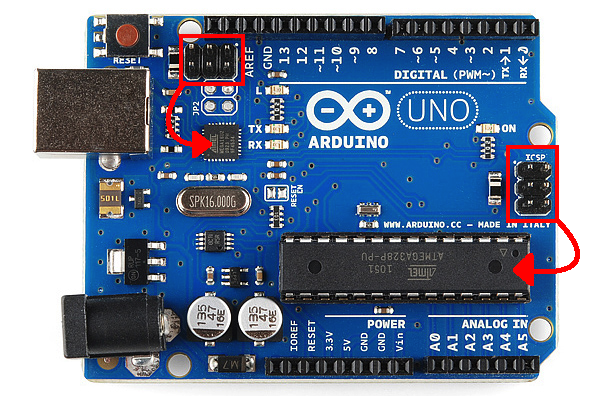
\includegraphics[scale=0.28]{images/arduino/isp}
    }
    \addtooverlay<.(1)>{
        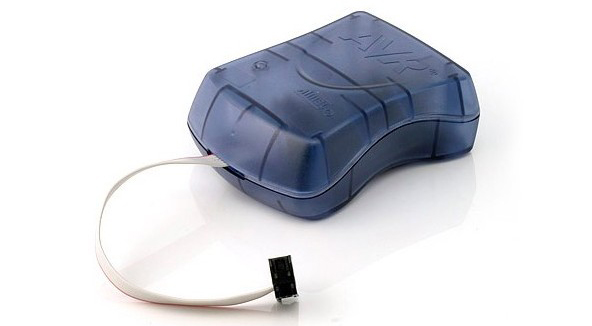
\includegraphics[scale=0.28]{images/avr-prog}
    }
    \addtooverlay<.(1)>{
        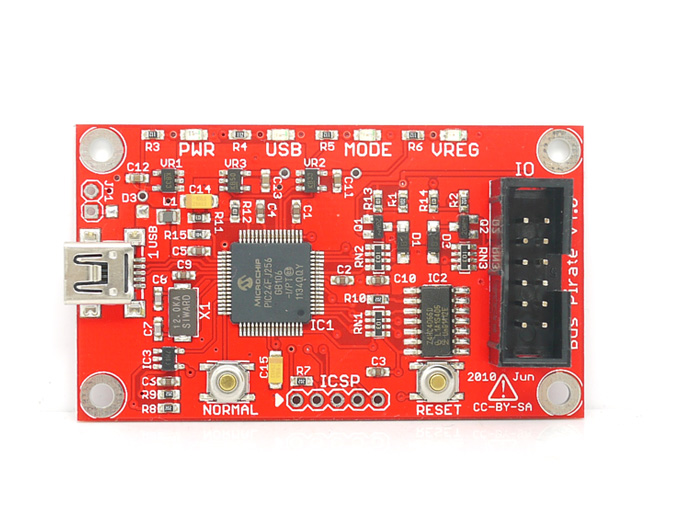
\includegraphics[scale=0.28]{images/bus-pirate}
    }
    \addtooverlay<.(1)>{
        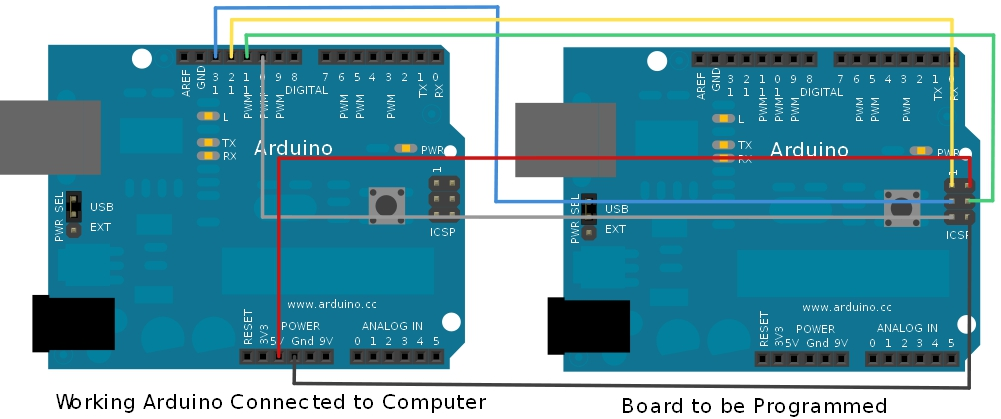
\includegraphics[scale=0.28]{images/arduino/prog}
    }
\end{frame}

\note[itemize] {
    \item Les cartes arduino disposent des connections ISP (pour programmation
        série in-situ) une pour le micro-controlleur lui même et une seconde
        pour celui qui gère l’usb.

    \item Toutefois il vous faudra un programmeur, il en existe des dédiés à
        cette tâche mais pour une utilisation occasionnelle.

    \item Je vous conseille plutôt le bus pirate qui poura servir à d’autres
        choses.

    \item Ou plus rigolo, utiliser un arduino pour programmer un autre arduino.

    \item Plutôt que de supprimer le bootloader, il est plus intéressant de
        chercher des alternatives. Par exemple tinysafeboot qui peux demander un
        mot de passe pour s’activer.
}
% }}}
% {{{ Le matériel
\begin{frame}
    \frametitle{Le matériel}
\end{frame}

\begin{frame}
    \frametitle{Le matériel}

    \addtooverlay<.(1)>{
        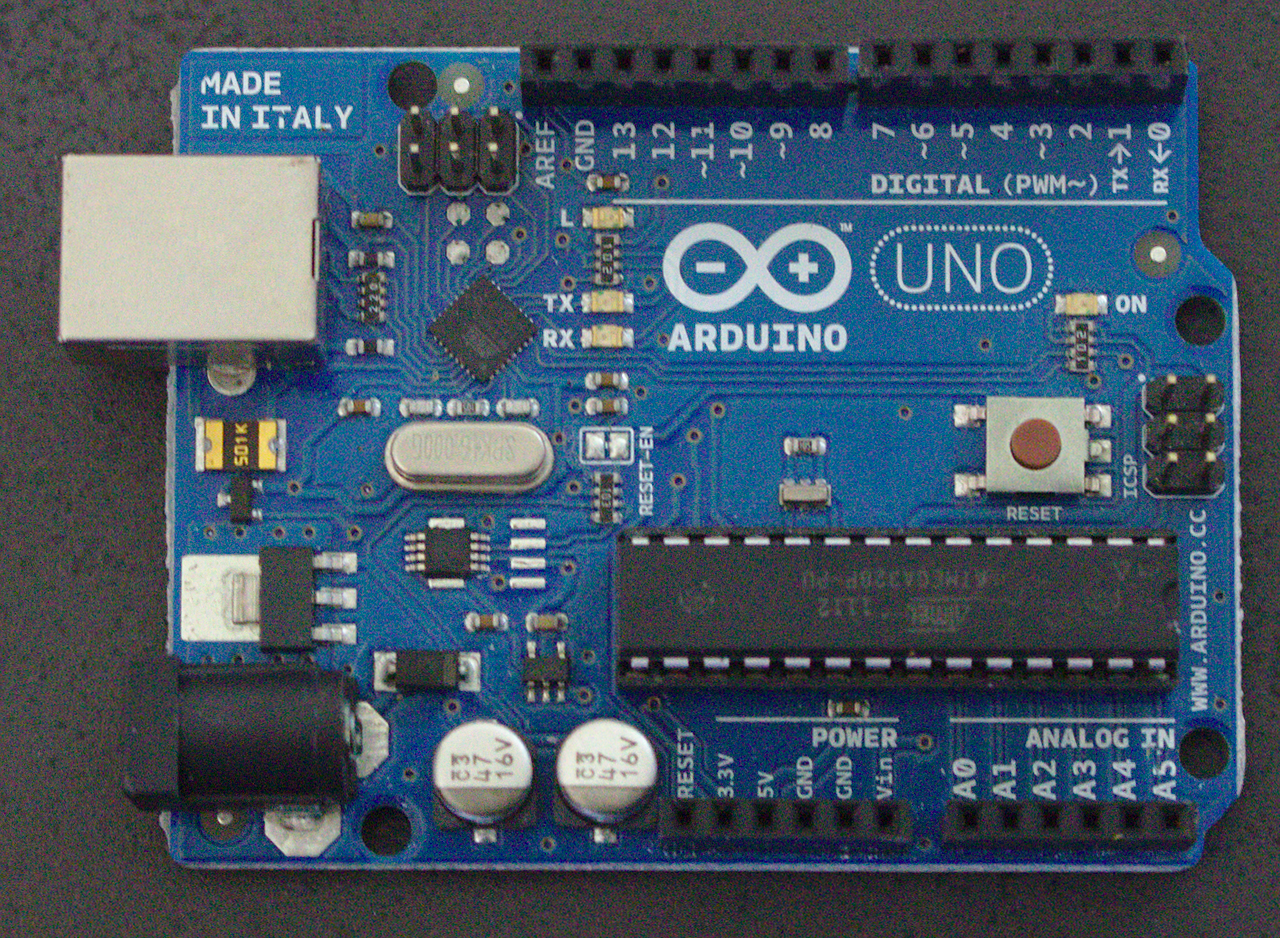
\includegraphics[scale=0.15]{images/arduino/uno}
    }
    \addtooverlay<.(1)>{
        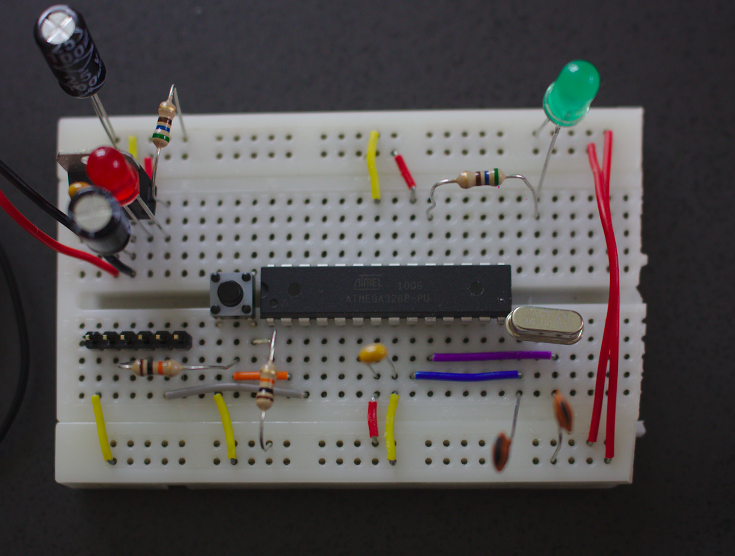
\includegraphics[scale=0.50]{images/arduino/destruct-1}
    }
    \addtooverlay<.(1)>{
        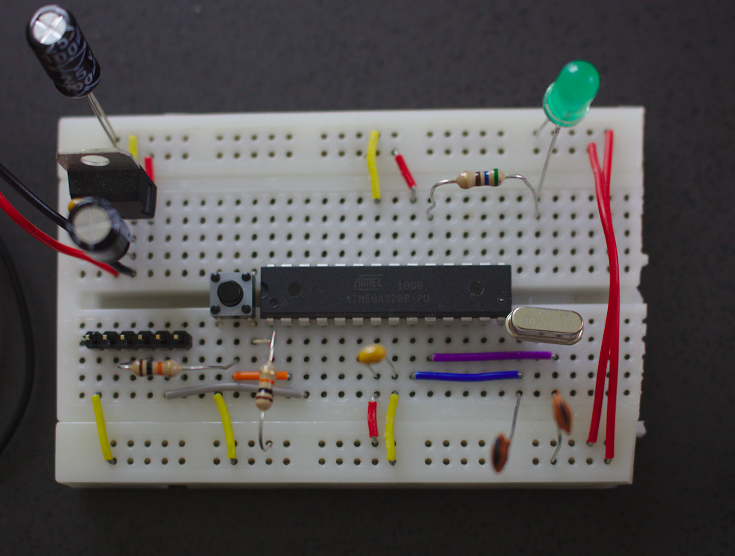
\includegraphics[scale=0.50]{images/arduino/destruct-2}
    }
    \addtooverlay<.(1)>{
        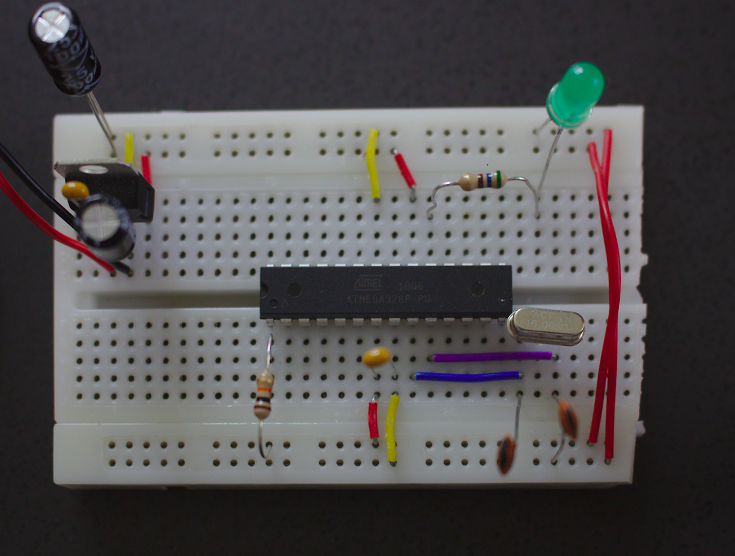
\includegraphics[scale=0.50]{images/arduino/destruct-3}
    }
    \addtooverlay<.(1)>{
        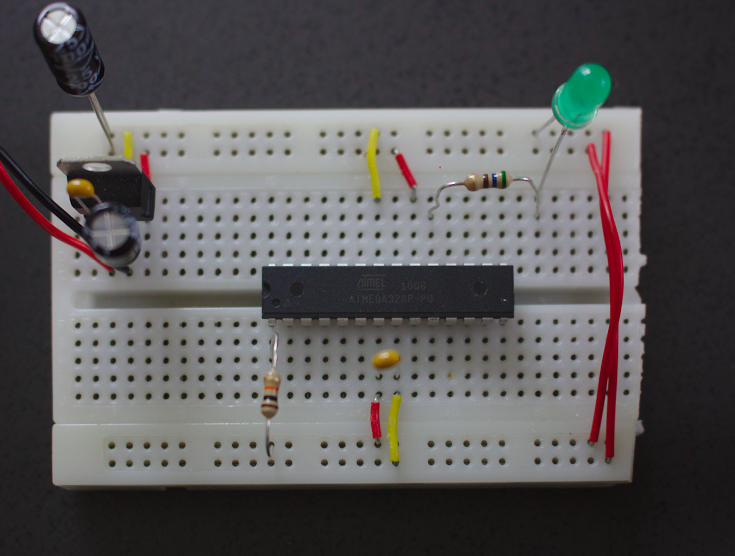
\includegraphics[scale=0.50]{images/arduino/destruct-4}
    }
\end{frame}

\note[itemize] {
    \item C’est un peu la même histoire qu’avec la partie logicielle : c’est
        pratique pour débuter mais c’est relativement lourd pour faire clignoter
        une led. Et là on parle d’une vingtaine d’euros par projet alors que le
        micro-controlleur coûte 3 euros.

    \item Il existe des kits pour construire un arduino sur une plaqe de
        developpement pour une dizaine d’heuro. Mais on peux encore supprimer
        des choses :

    \item la led de l’alimentation ;
    \item la partie programmation et le bouton reset ;
    \item l’oscillateur. Car l’atmega possède un cristal interne à 8MHz. On a
        encore diviser par deux le prix de notre montage pour arriver à 5 euros. Et
        ce n’est pas fini.
}

\begin{frame}
    \frametitle{Le matériel}

    \addtooverlay<.(1)>{
        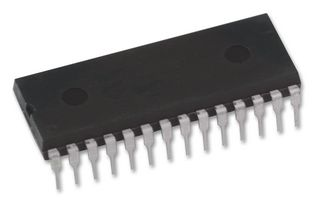
\includegraphics[scale=0.40]{images/arduino/atmega}
    }
    \addtooverlay<.(1)>{
        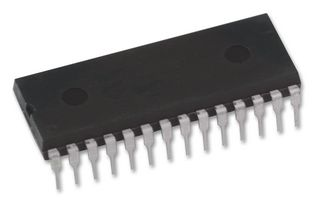
\includegraphics[scale=0.40]{images/arduino/atmega}
        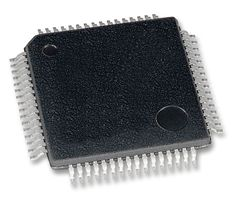
\includegraphics[scale=0.40]{images/arduino/atxmega}
    }
    \addtooverlay<.(1)>{
        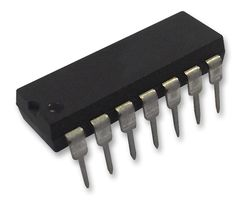
\includegraphics[scale=0.40]{images/arduino/attiny}
        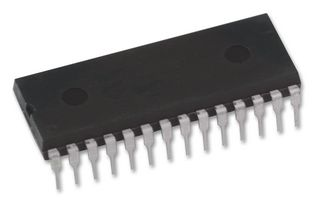
\includegraphics[scale=0.40]{images/arduino/atmega}
        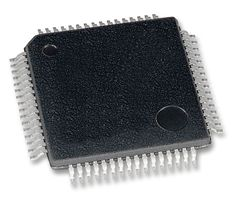
\includegraphics[scale=0.40]{images/arduino/atxmega}
    }
\end{frame}

\note[itemize] {
    \item Atmel propose plusieurs ici nous avons utilisé un megaAVR.

    \item La seconde famille plus puissante, les xmega que l’on retrouve dans
        les arduino mega.

    \item Mais il existe une troisième famille, moins puissante et donc moins
        chère, les attiny. Cela permet de diviser encore par deux les prix. Un
        attiny côute moins de 2 euros.

    \item Une fois que vous avez réalisez votre circuit sur une plate forme de
        dev, il est temps de passer à la version finale sur un circuit imprimé.
}
% }}}
% }}}

\begin{frame}
    \addtooverlay<.(1)>{
        
\includegraphics[scale=0.15]{images/ghs}
    }
\end{frame}

\note[itemize] {
    \item Petite paranthèse pour vous éviter une nomination au Darwing auwards,
        dans les deux prochaines parties il va être questions de produits
        chimiques. Lisez bien les embalages avant de jouer avec. Il y a des
        pictogrammes comme celui-ci qui vous permettent rapidement savoir à quoi
        vous vous exposez.
    \item Protégez les yeux avec des lunettes adapatées, qui couvrent également
        sur le côté.
    \item Une blouse, pas uniquement pour protéger vos vêtements, mais une
        blouse en coton qui vous protégera en cas de brulure (par du feu ou de
        l’acide).
    \item Et éviter les gants, car s’ils prennent feu, ils ont la mauvaise idée
        de resté coller à vos mains. Les gars sont nécessaires lorsqu’on
        manipule des produits biologiques (comme du sang) ou mutagènes.
}

% {{{ Circuit imprimé
\section{Circuit imprimé}
\begin{frame}
    \tableofcontents[currentsection]
\end{frame}

\note[itemize] {
    \item J’avais en tête la méthode de labo, compliquée et qui demande du
        matériel.  Il existe des méthodes plus simples, en particulier pour
        l’insolation.
}
% {{{ Préparation
\begin{frame}
    \frametitle{Préparation}

    \addtooverlay<.(1)>{
        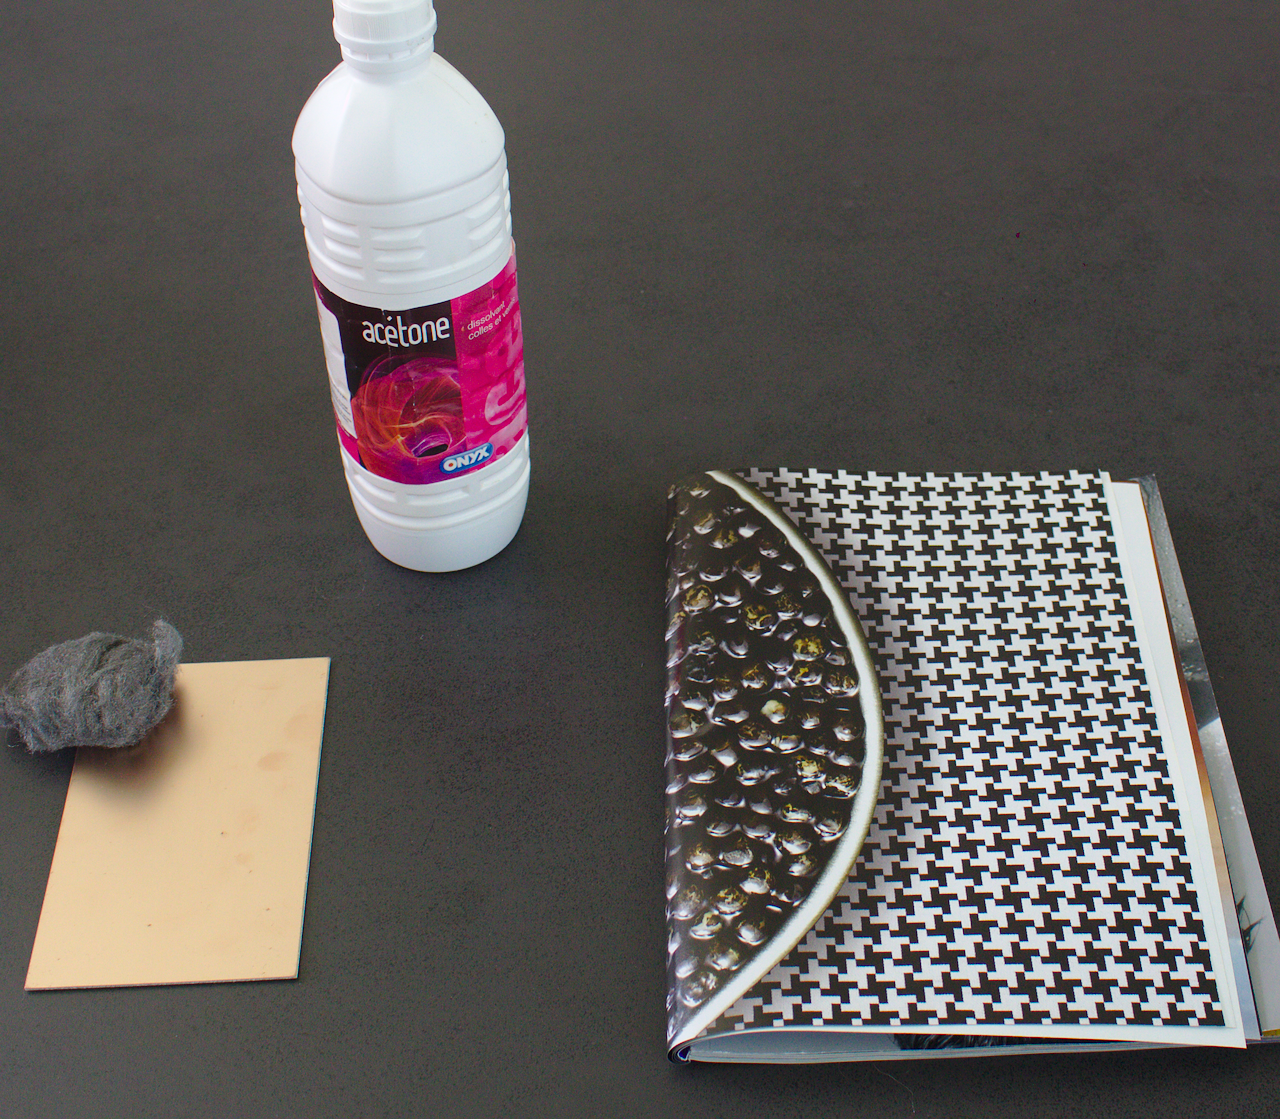
\includegraphics[scale=0.15]{images/pcb/preparation}
    }
\end{frame}

\note[itemize] {
    \item Une fois la plaque, non sensibilisée, découpée au format du typon, on
        raille légèrement la surface avec de la paille de fer puis on la netoye
        avec de l’acétone.
}
% }}}
% {{{ Transfert à chaud
\begin{frame}
    \frametitle{Transfert à chaud}

    \addtooverlay<.(2)>{
        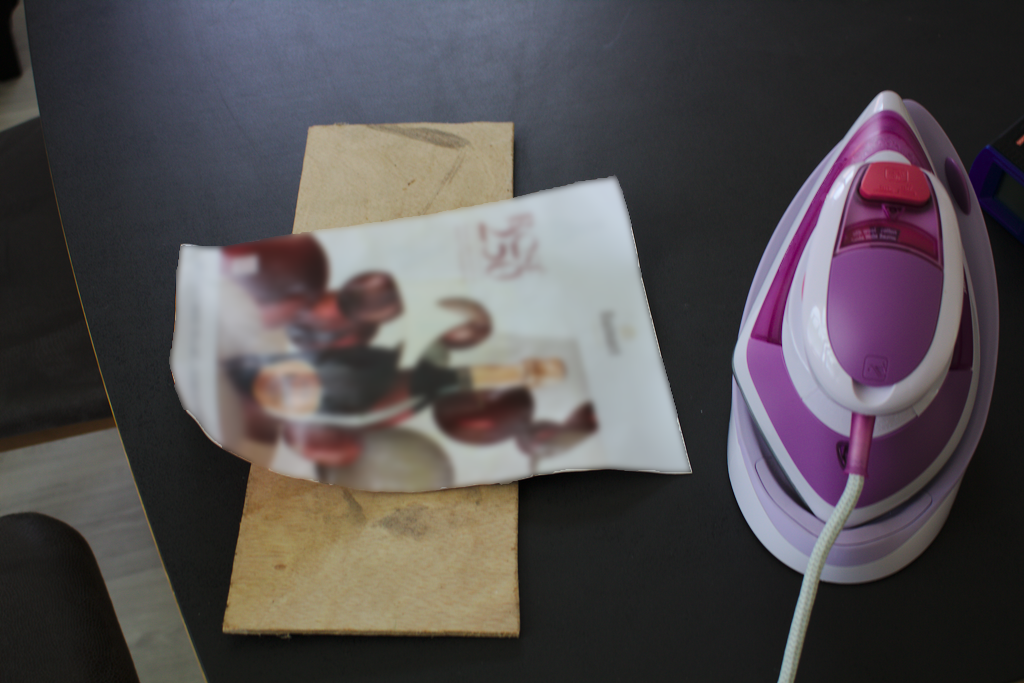
\includegraphics[scale=0.28]{images/pcb/fer}
    }
    \addtooverlay<.(2)>{
        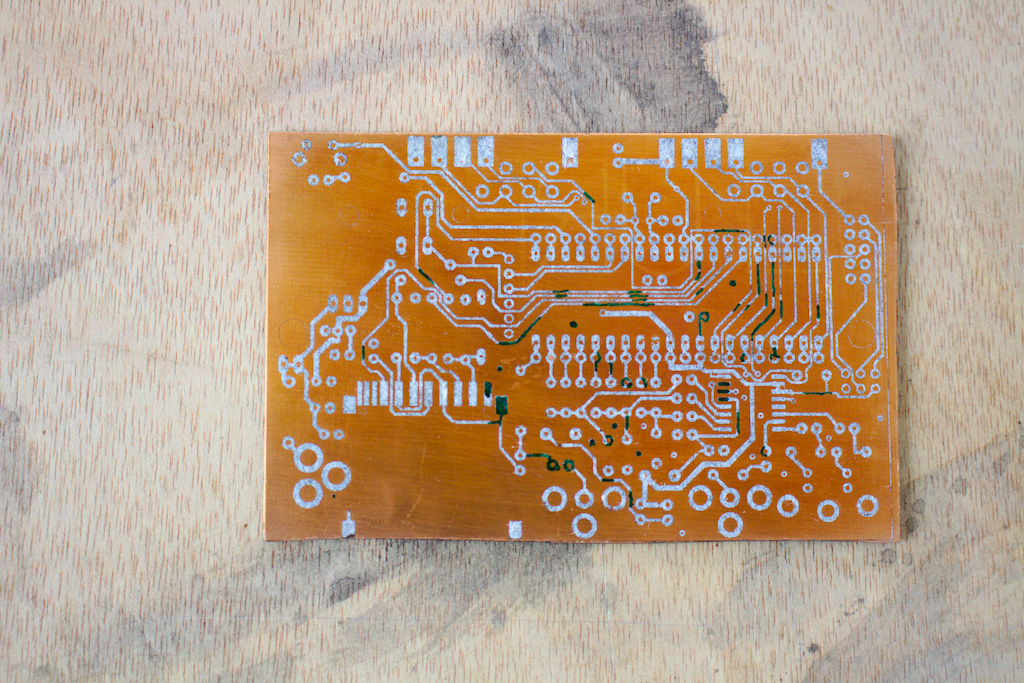
\includegraphics[scale=0.28]{images/pcb/fer2}
    }
\end{frame}

\note[itemize] {
    \item Première méthode de transfert, avec un fer à repassé. Il suffit
        d’imprimer le typon sur un papier glacé de mauvaise qualité avec une
        imprimante laser.

    \item On l’applique sur une plaque en appuyant pendant 15 minutes environ.

    \item Une fois la plaque refrodie, il suffit le retirer délicatement la
        feuille. Éventuellement compléter les pistes avec un marqueur.
}
% }}}
% {{{ Transfert à froid
\begin{frame}
    \frametitle{Transfert à froid}

    \begin{itemize}
        \item<1-> Alcool 8/11
        \item<1-> Acétone 3/11
    \end{itemize}
\end{frame}

\note[itemize] {
    \item Avec une solution d’alcool et d’acétone dans un rapport 8 pour 3.

    \item Dans tous les cas, si vous vous êtes trompé de sens pour le typon, un
        coup d’acétone et on recommence.
}
% }}}
% {{{ Gravure
\begin{frame}
    \frametitle{Gravure}
\end{frame}

\note[itemize] {
    \item Maintentant, on va graver le circuit, c’est à dire enlever la couche
        de cuivre sur les parties qui ne sont pas protégées par te tonner.
}

\begin{frame}
    \frametitle{Gravure}

    \addtooverlay<.(1)>{
        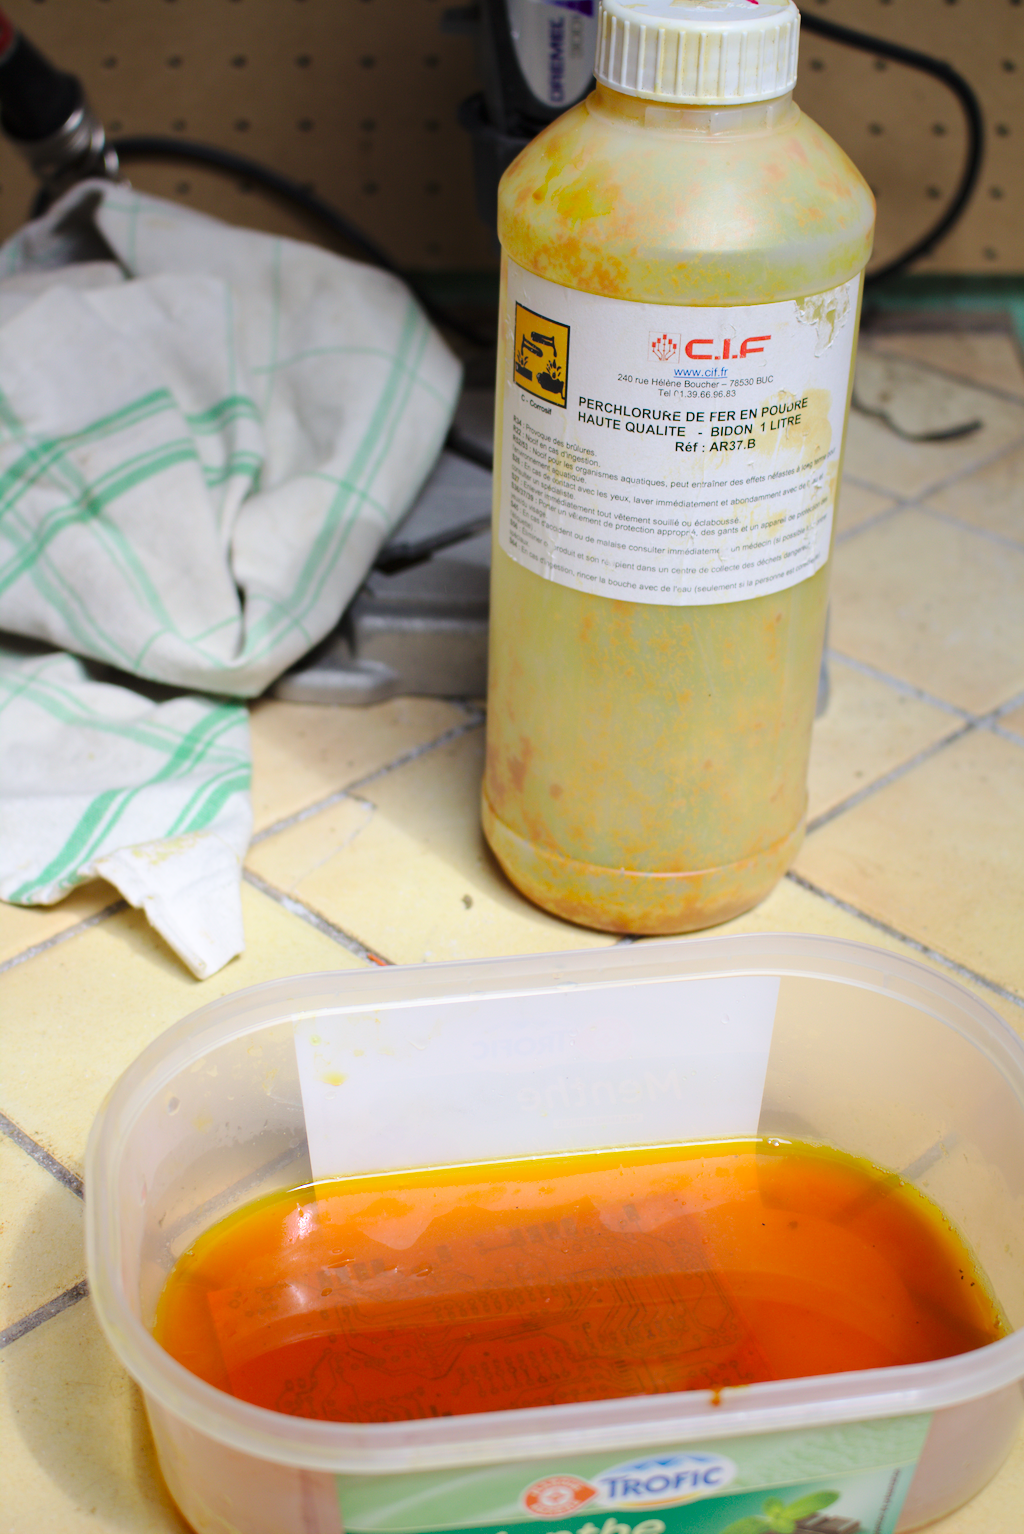
\includegraphics[scale=0.14]{images/pcb/perchlo}
    }
    \addtooverlay<.(1)>{
        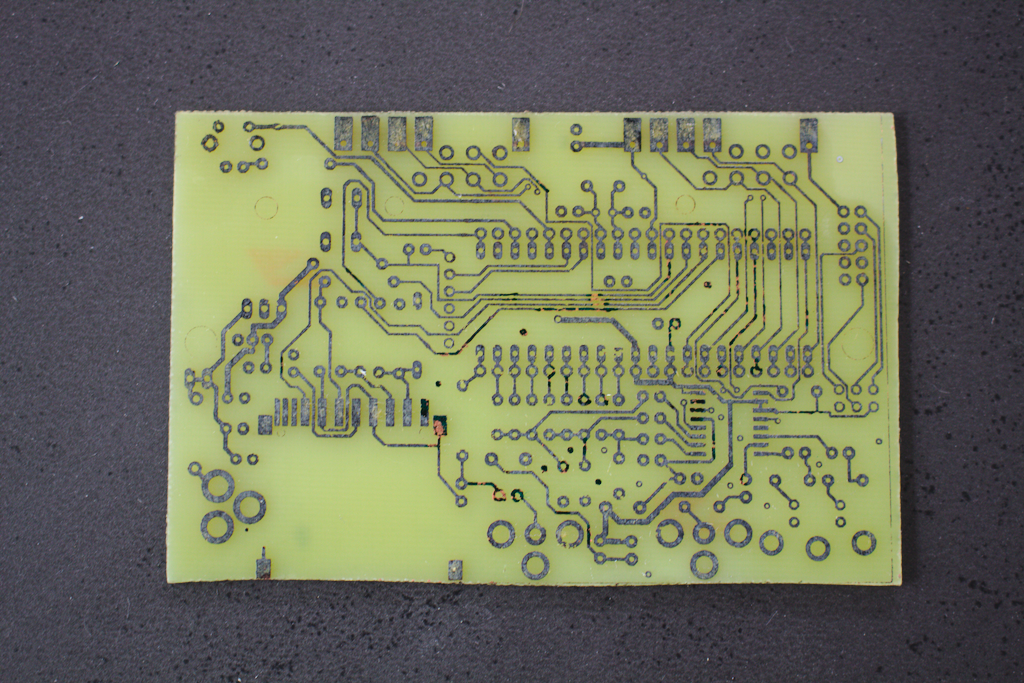
\includegraphics[scale=0.28]{images/pcb/perchlo2}
    }
    \addtooverlay<.(1)>{
        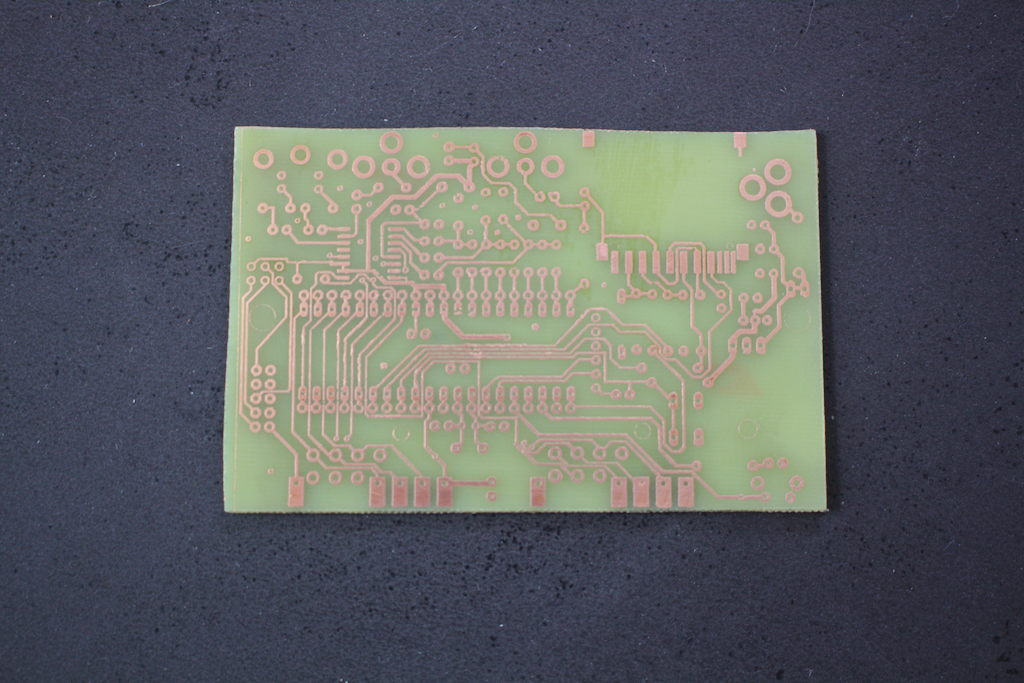
\includegraphics[scale=0.28]{images/pcb/final}
    }
    \addtooverlay<.(1)>{
        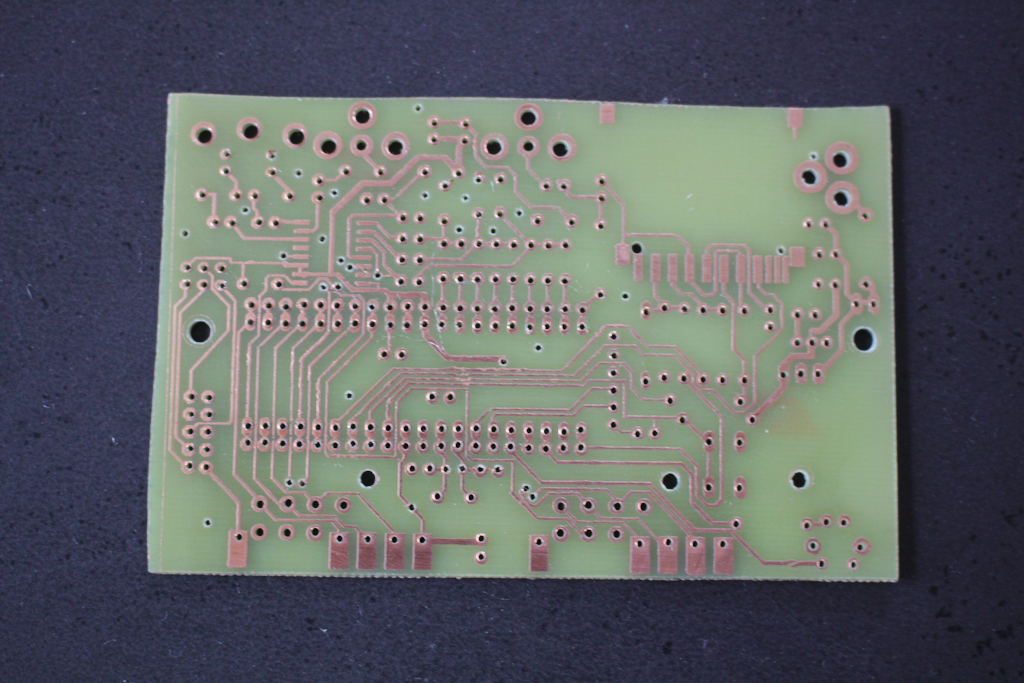
\includegraphics[scale=0.28]{images/pcb/trous}
    }
\end{frame}

\note[itemize] {
    \item C’est la partie sale qui nécessite du perchlorure de fer : en plus
        d’être corosif ça tâche. On dissous le perchlo dans de l’eau tiède. On
        laisse tremper trois quart d’heure - une heure en remuant de temps en temps.

    \item Voici le résultat une fois rincé à l’eau.

    \item Un petit coup d’acétone pour nettoyer les pistes.

    \item Et on termine par percer les trous.
}
% }}}
% }}}

% {{{ CMS
\section{CMS}
\begin{frame}
    \tableofcontents[currentsection]
\end{frame}

\note[itemize] {
    \item CMS pour composant monté en surface
}

\begin{frame}
    \addtooverlay<.(1)>{
        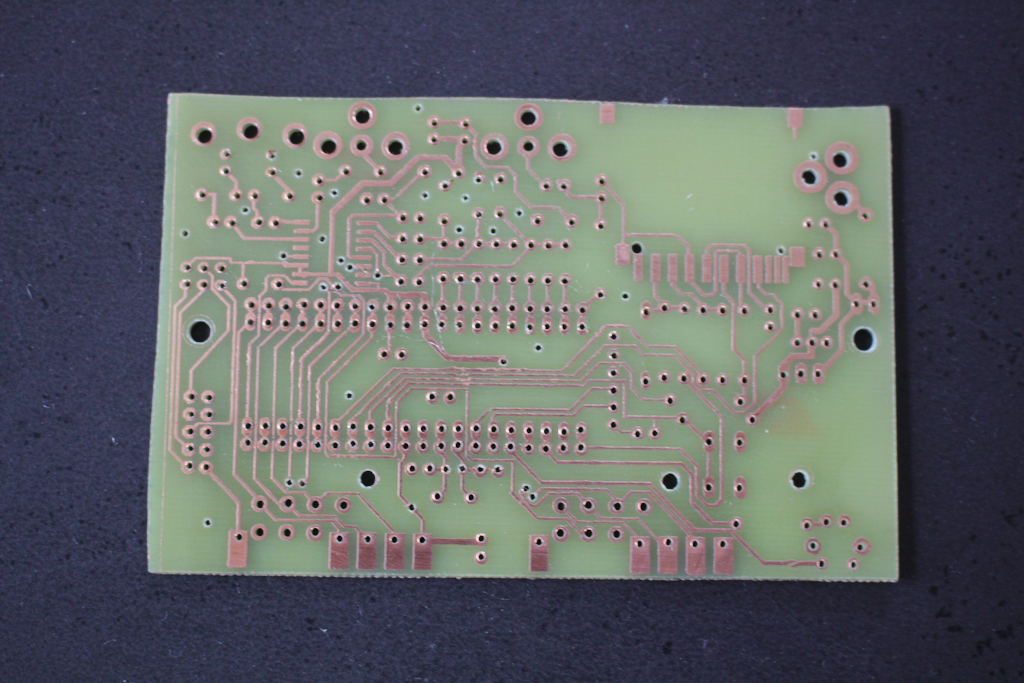
\includegraphics[scale=0.28]{images/pcb/trous}
    }
\end{frame}

\note[itemize] {
    \item Pourquoi soudé en surface ? Parce que vous risquez de ne pas avoir le
        choix, si vous reprenner des schéma open-hardware et à mon niveau, c’est
        sourtout que faire des trous ça devient vite pénible.
}

\begin{frame}
    \addtooverlay<.(1)>{
        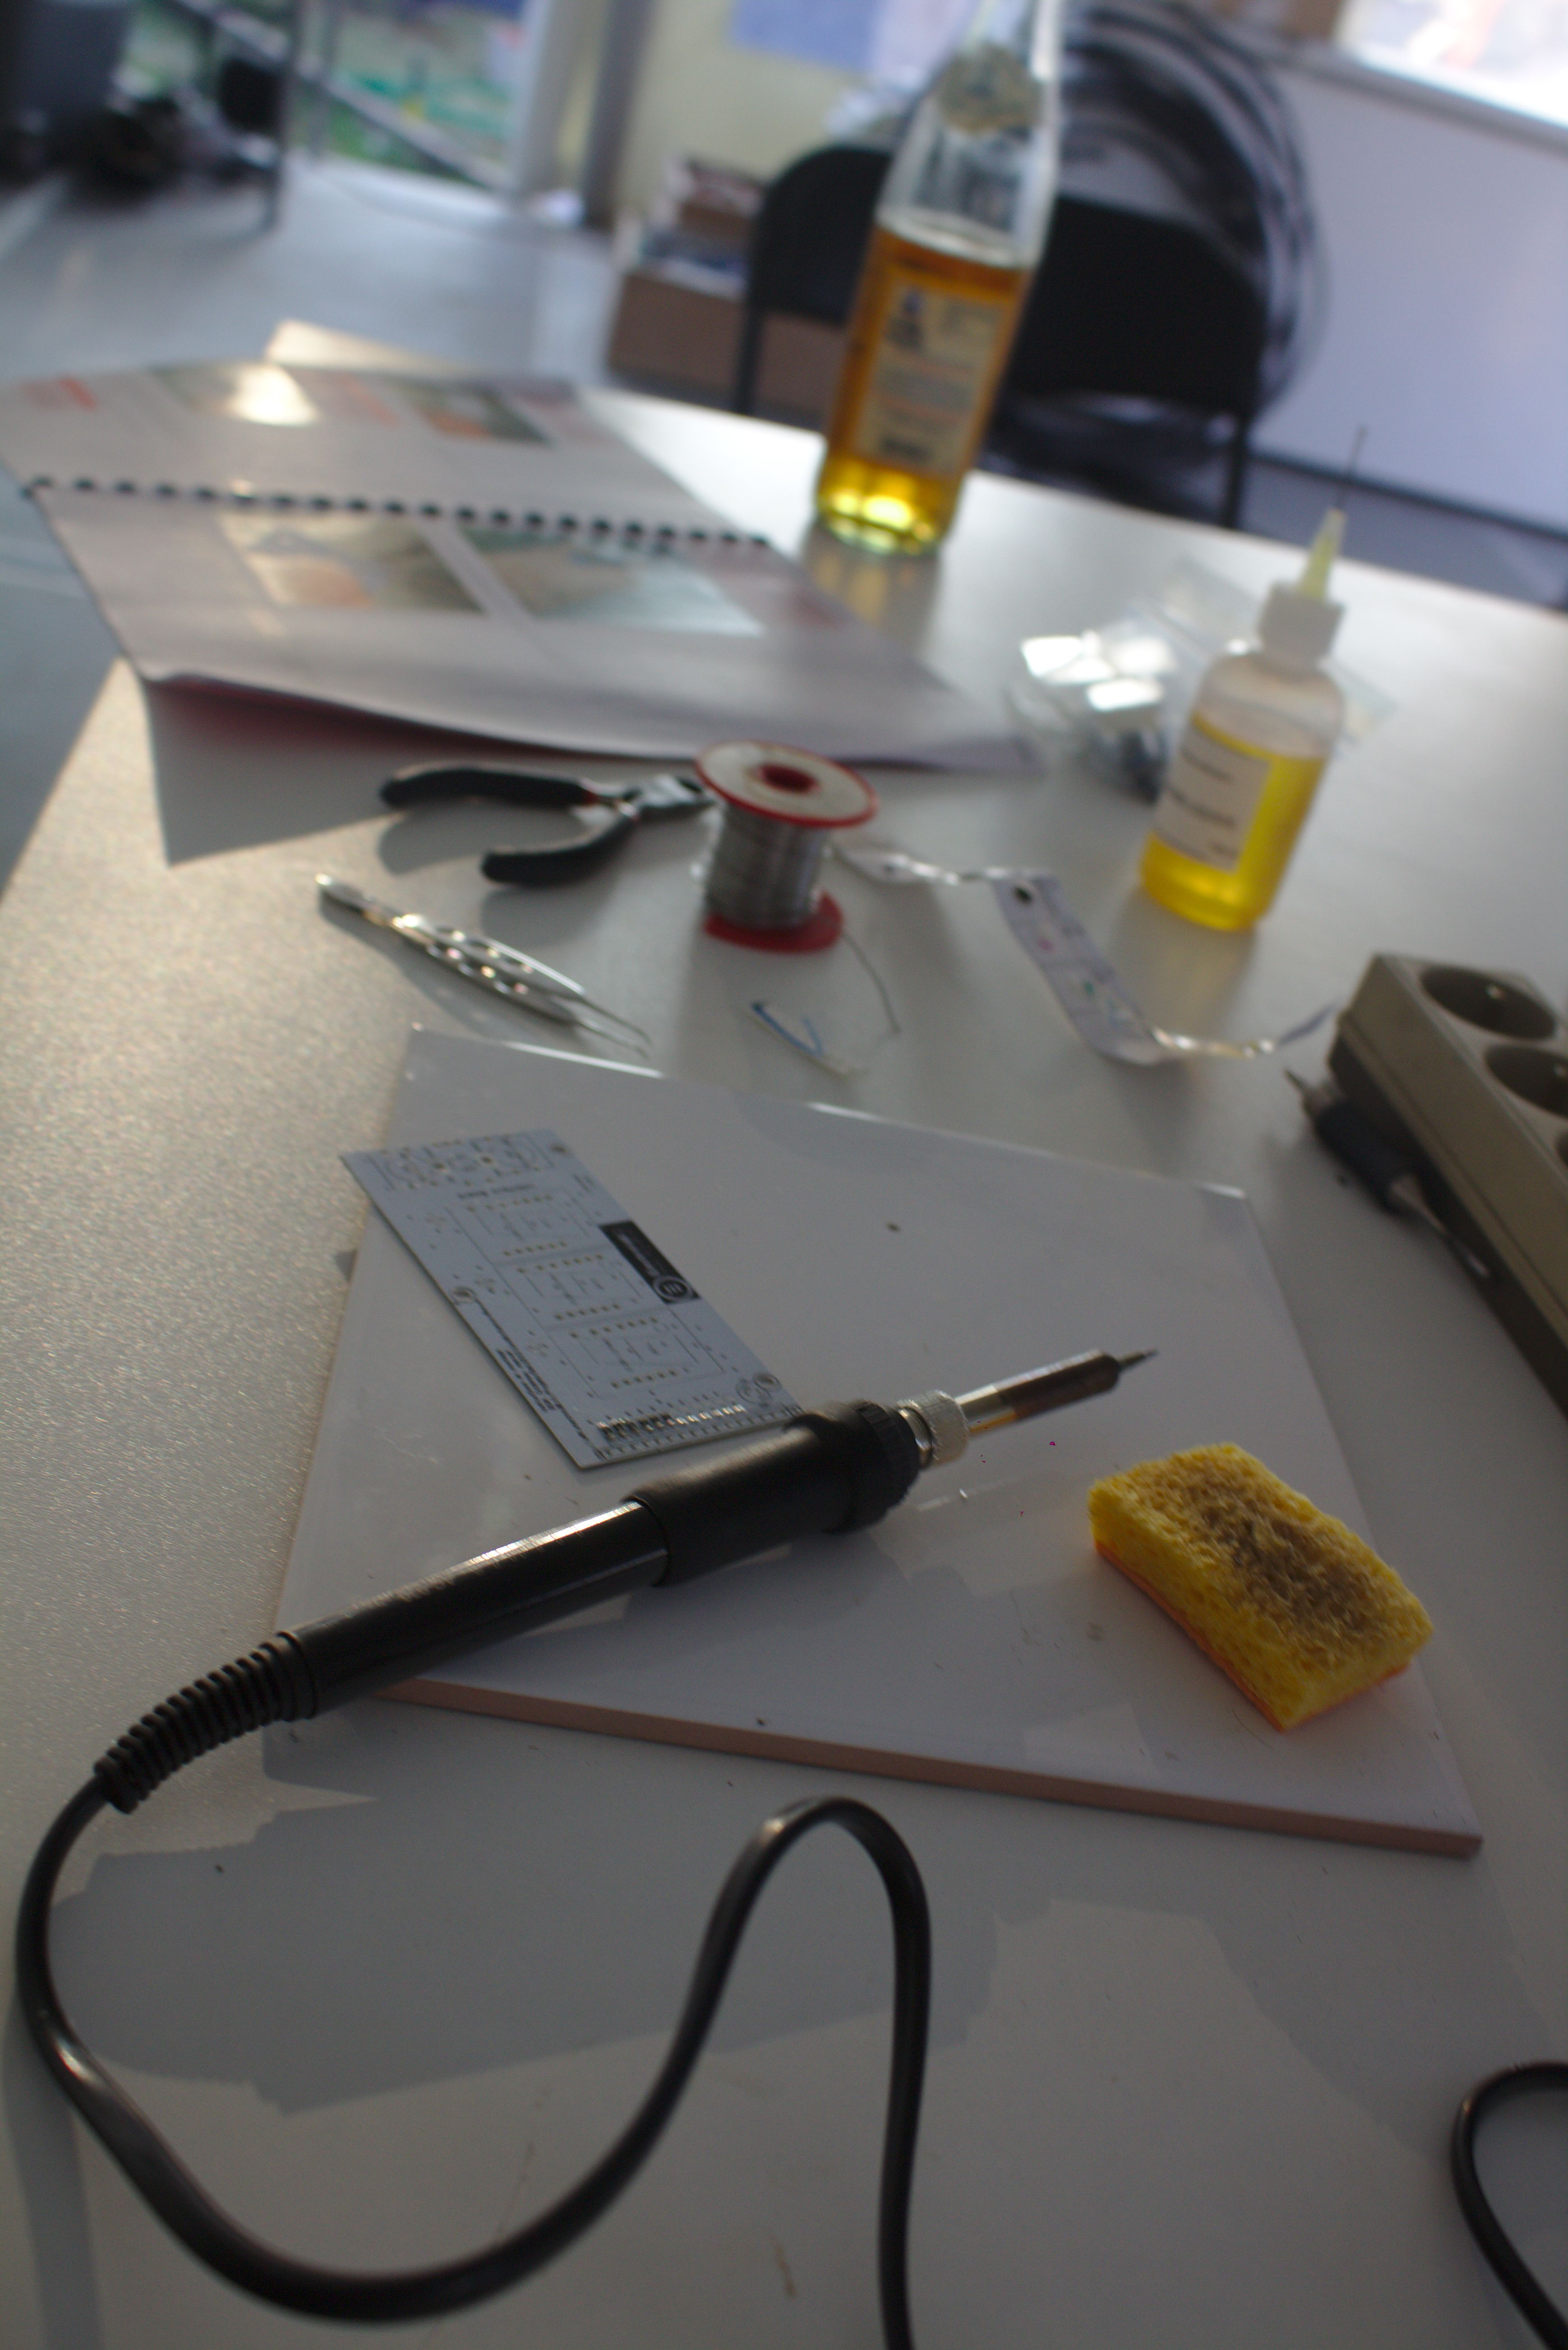
\includegraphics[scale=0.20]{images/smd/all}
    }
    \addtooverlay<.(1)>{
        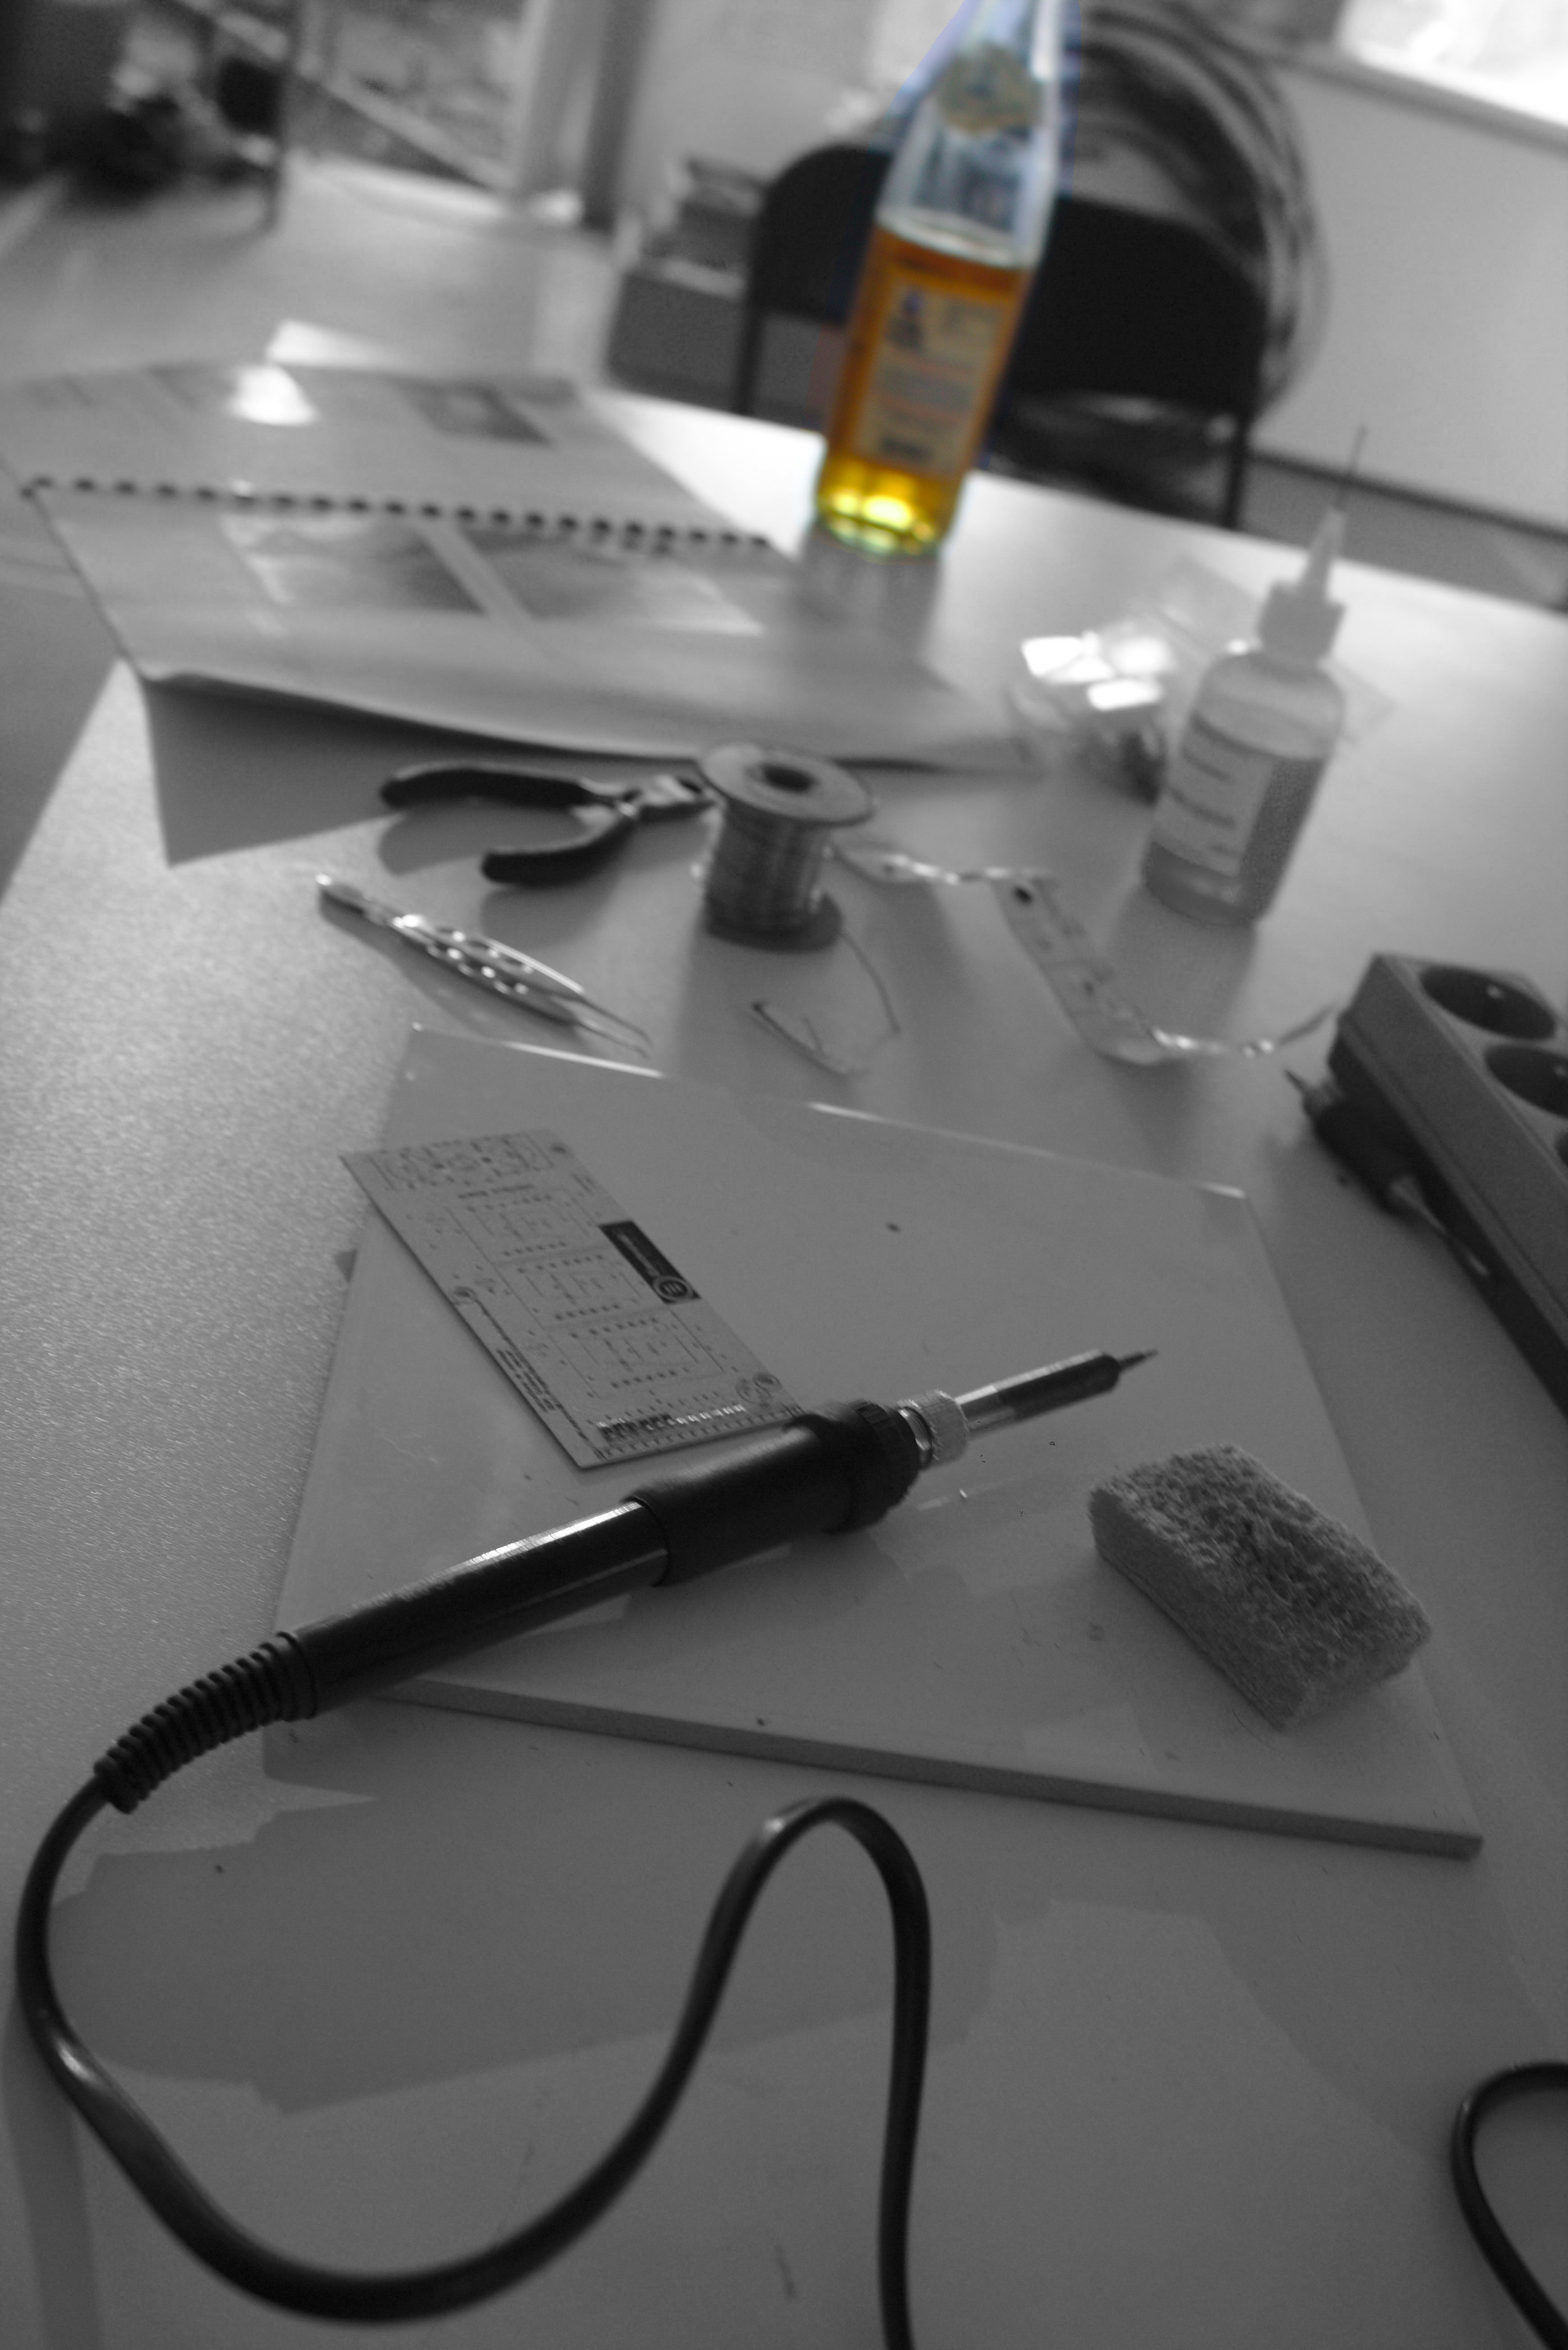
\includegraphics[scale=0.20]{images/smd/mate}
    }
    \addtooverlay<.(1)>{
        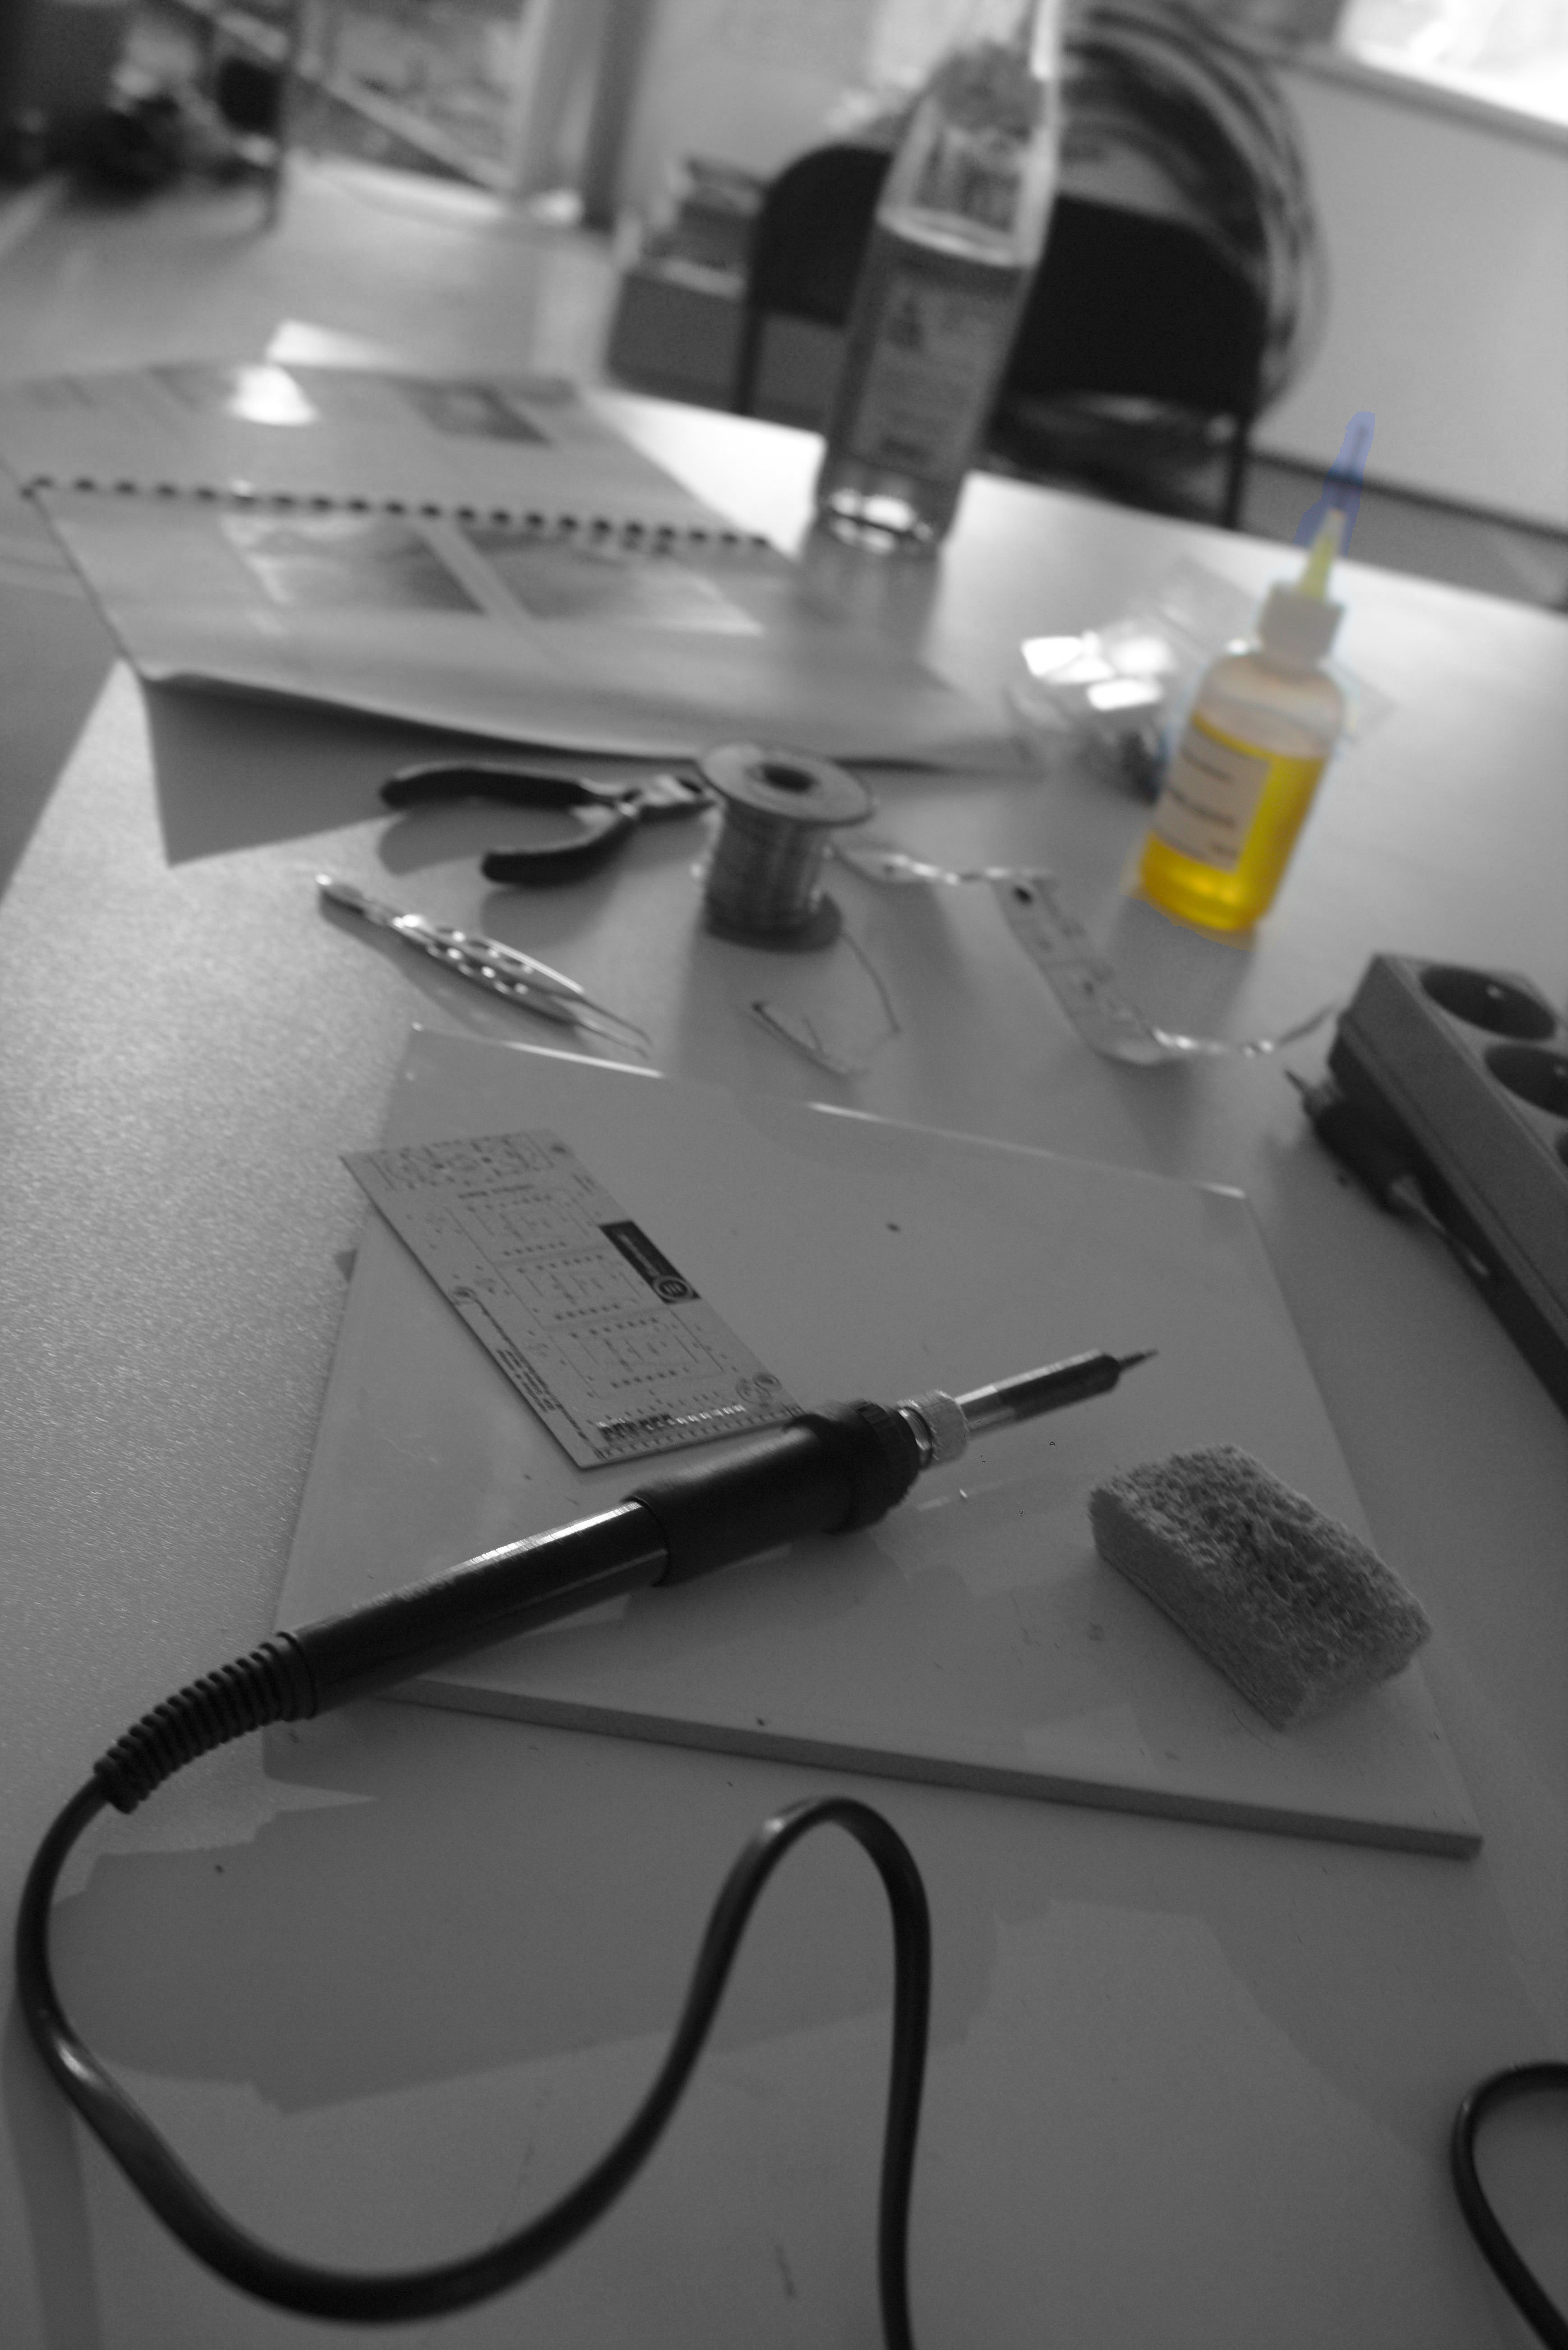
\includegraphics[scale=0.20]{images/smd/flux}
    }
    \addtooverlay<.(1)>{
        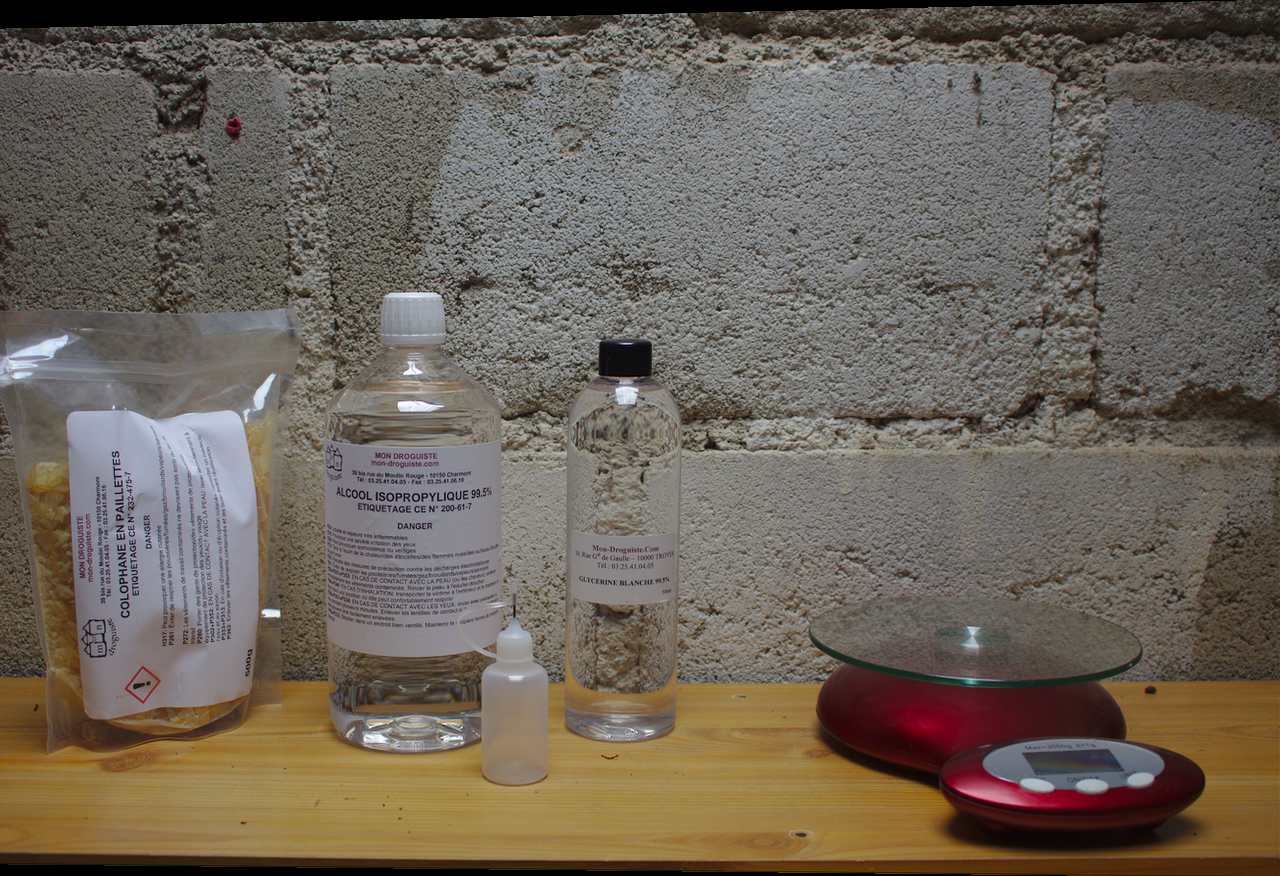
\includegraphics[scale=0.20]{images/smd/flux-diy}
    }
    \addtooverlay<.(1)>{
        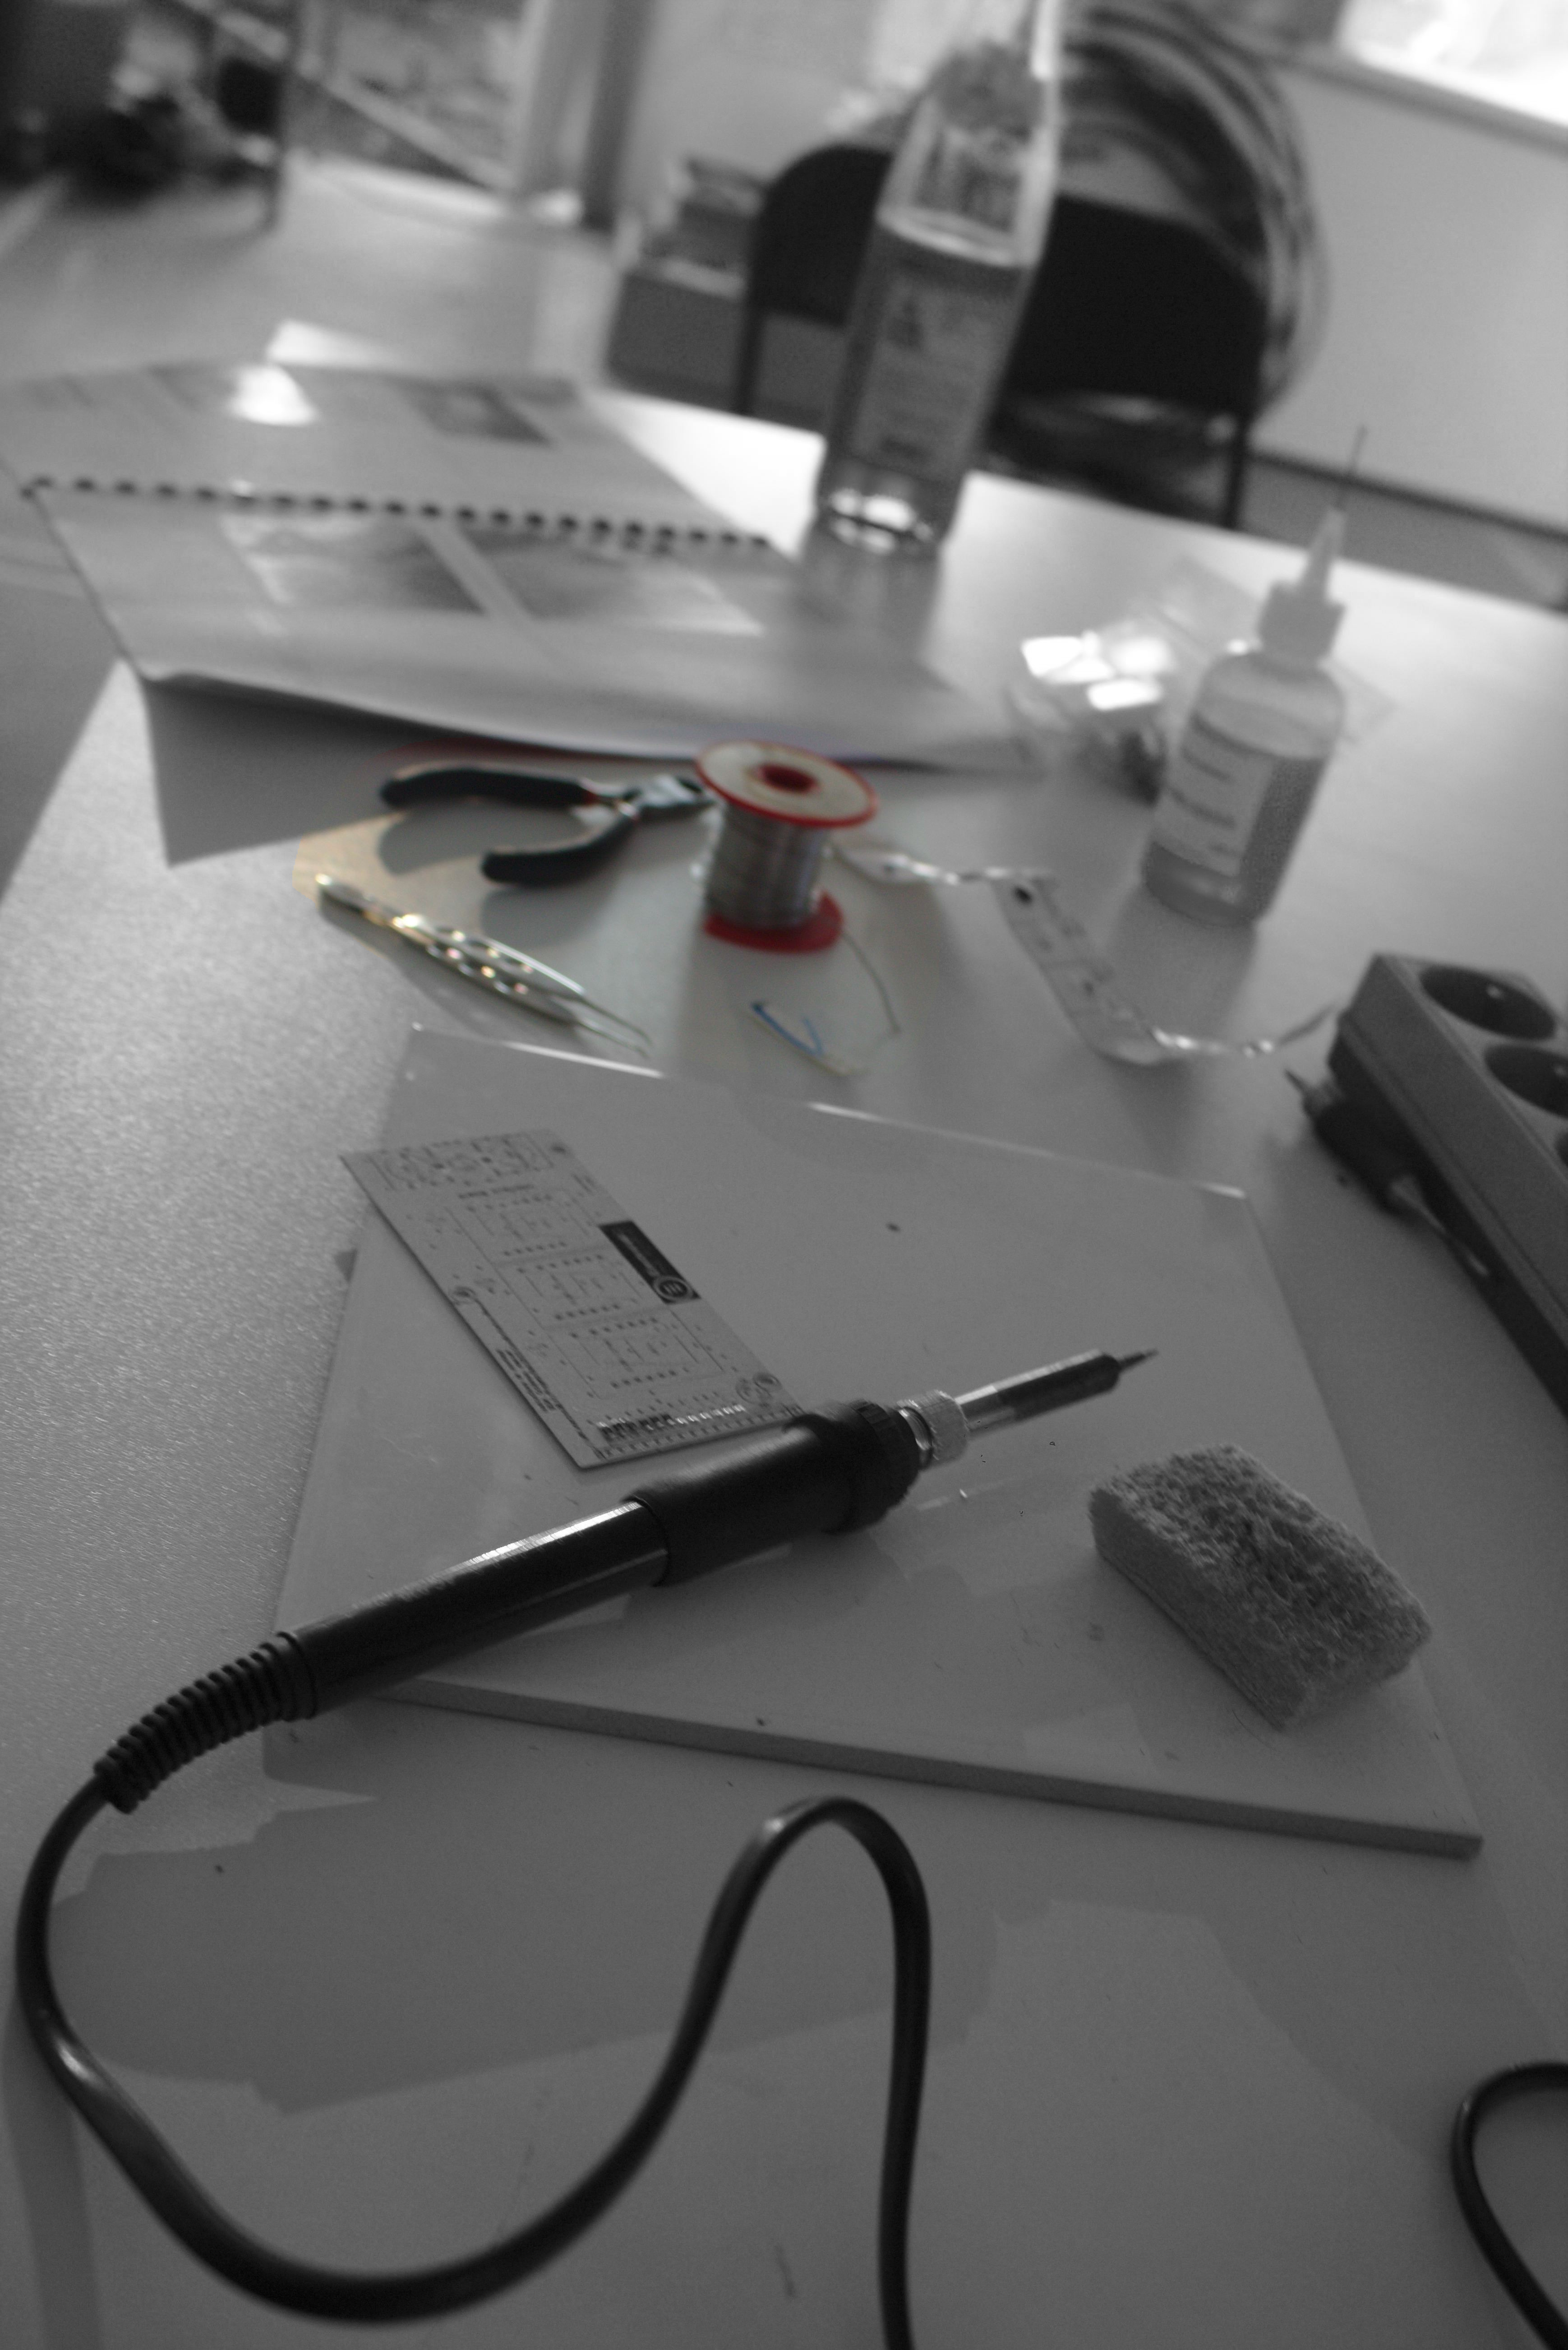
\includegraphics[scale=0.20]{images/smd/outils}
    }
    \addtooverlay<.(1)>{
        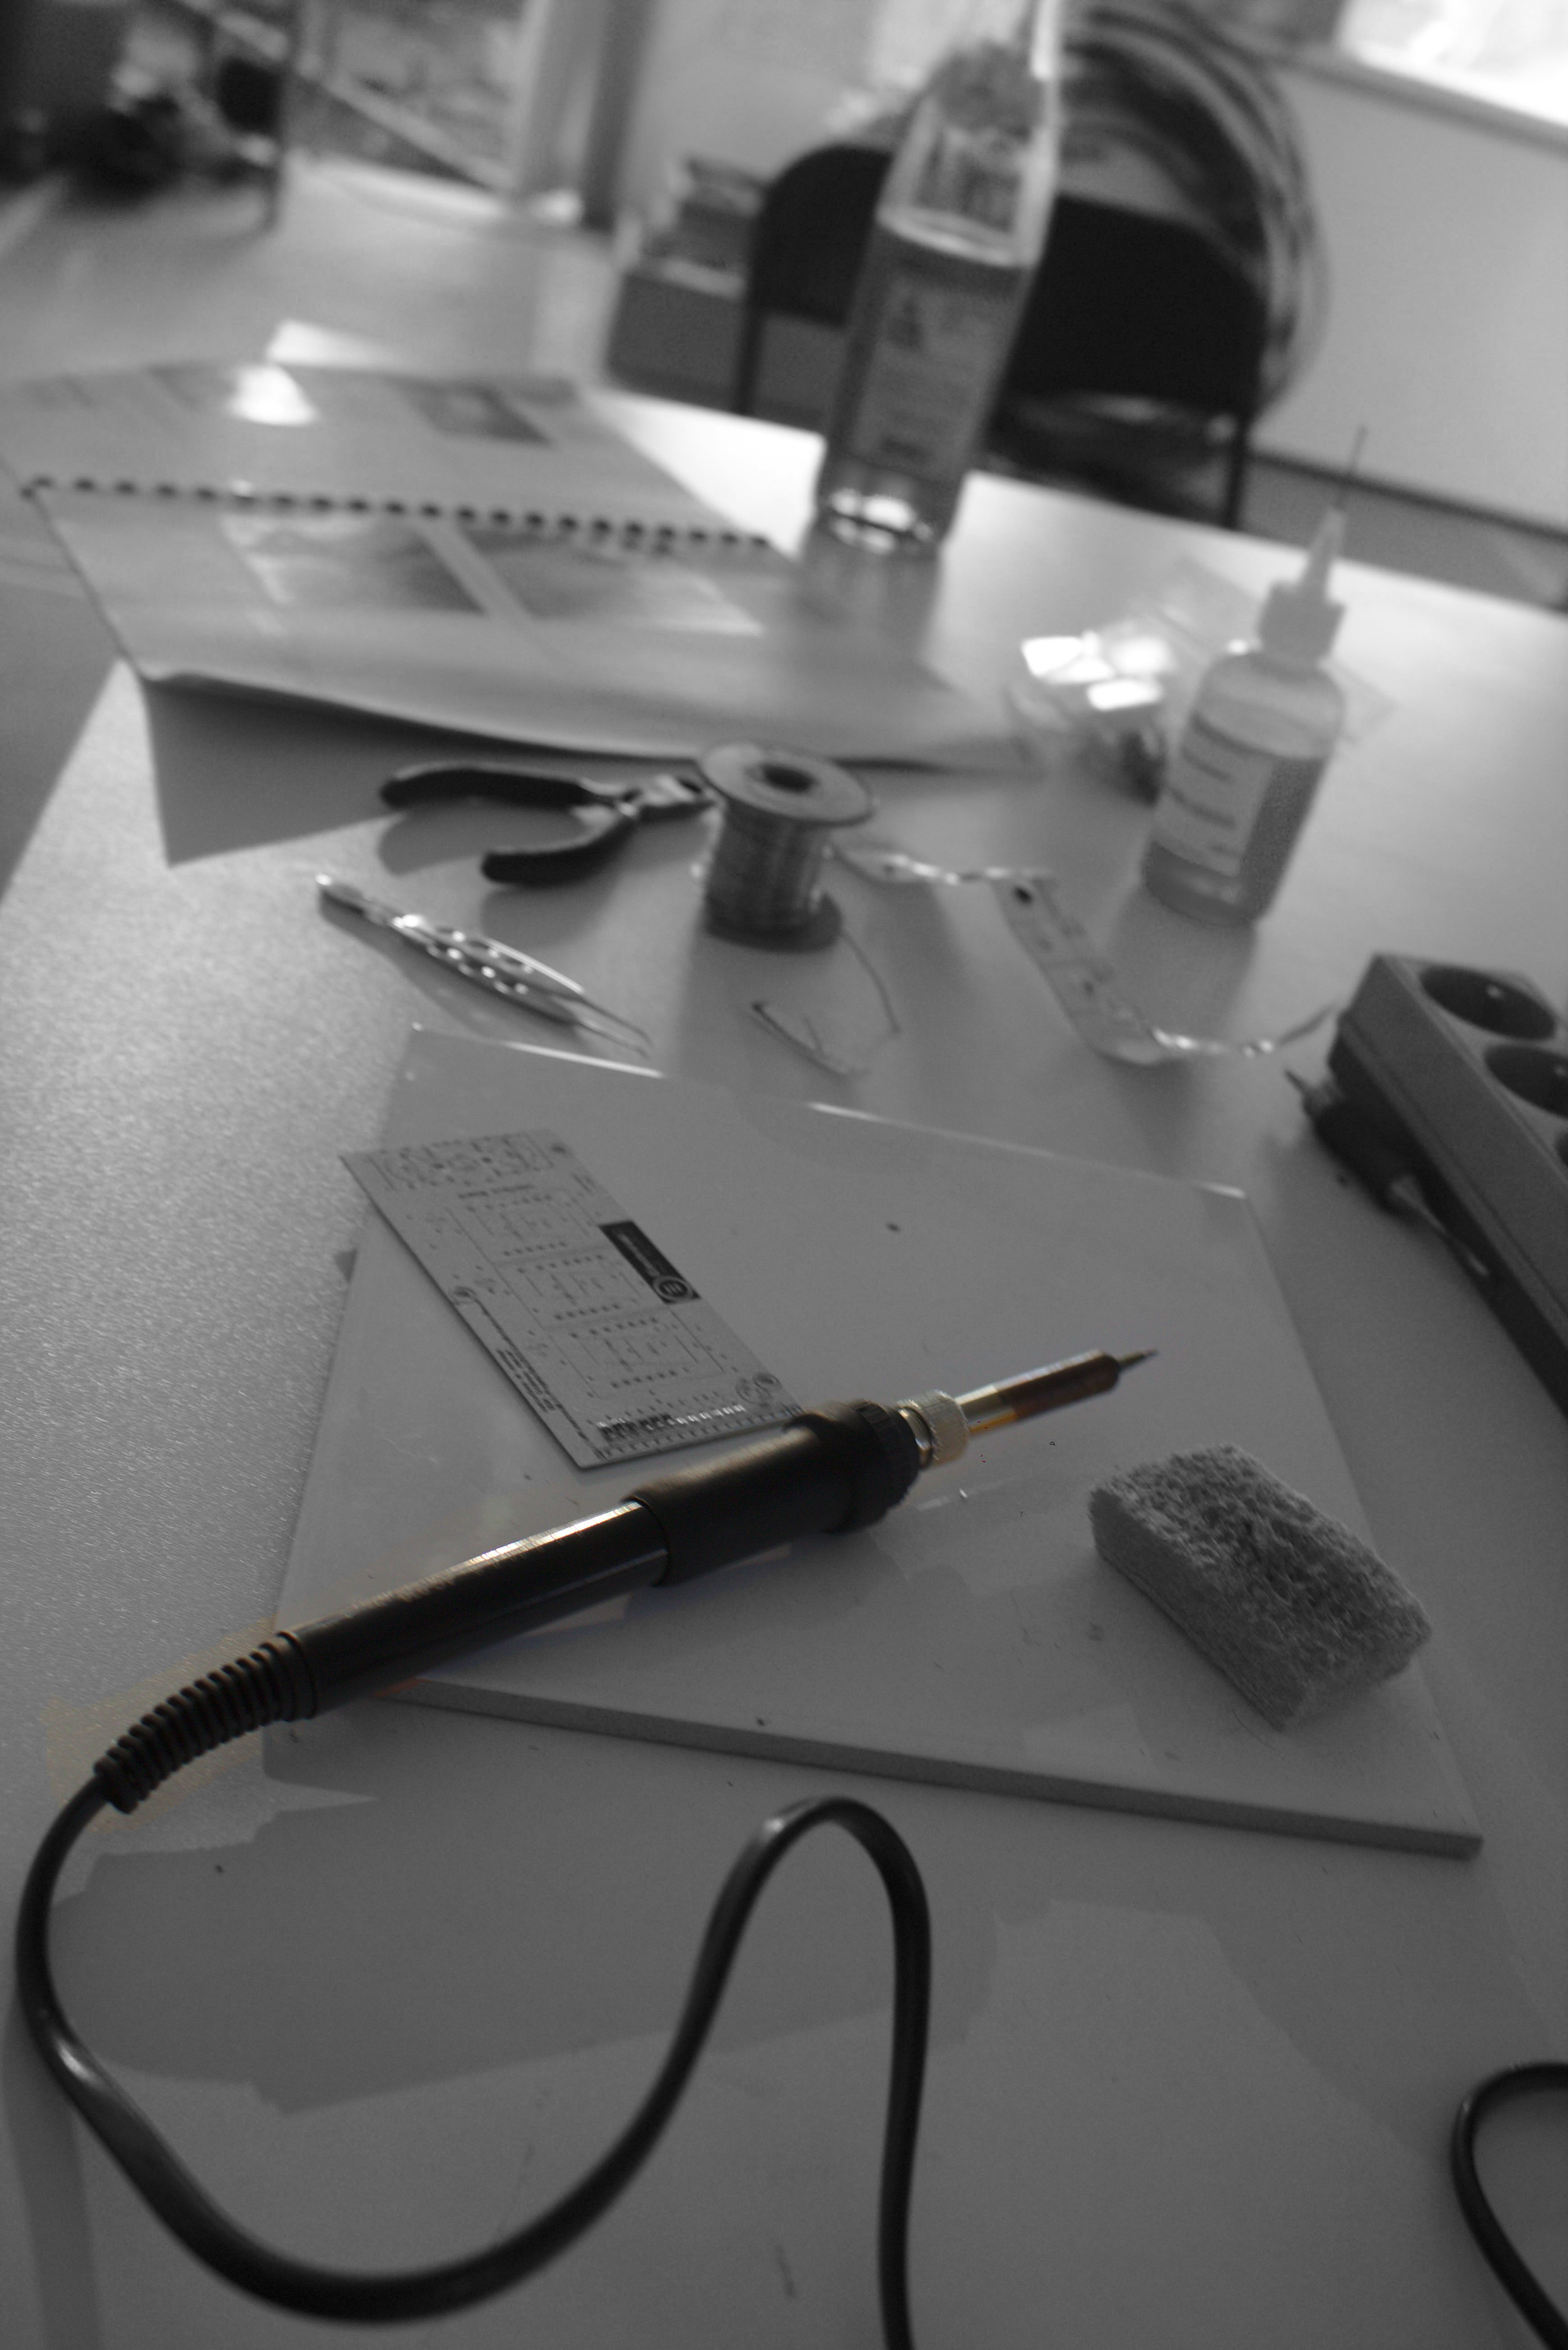
\includegraphics[scale=0.20]{images/smd/fer}
    }
\end{frame}

\note[itemize] {
    \item Du plus important au moins important :

    \item Du maté ;

    \item  Du flux : c’est l’ingrédient magique qui va faire que l’étain va
        adhéré uniquement aux parties métaliques.

    \item Vous pouvez l’acheter tout fait ou vous amuser à le faire avec du
        colophane (résine de pin), de l’alcool isopropylique et de la glycérine.

    \item De l’étain, mais surtout une pince pour tenir de petit objet ;

    \item Et enfin un fer. Un simple fer, il n’est pas nécessaire d’avoir une
        station.

    \item Si vous souhaitez essayer, tout est documenté sur le wiki de
        l’electrolab. Tous les liens sont en fin de diaporama.
}
% }}}

% {{{ FPGA
\section{FPGA}
\begin{frame}
    \tableofcontents[currentsection]
\end{frame}

\note[itemize] {
    \item Pour finir, j’aimerai vous parler d’un domaine de l’électronique que
        j’ai découvert il y a peu de temps : les FPGA.
}

\begin{frame}
    \frametitle{FPGA}

    \addtooverlay<.(1)>{
        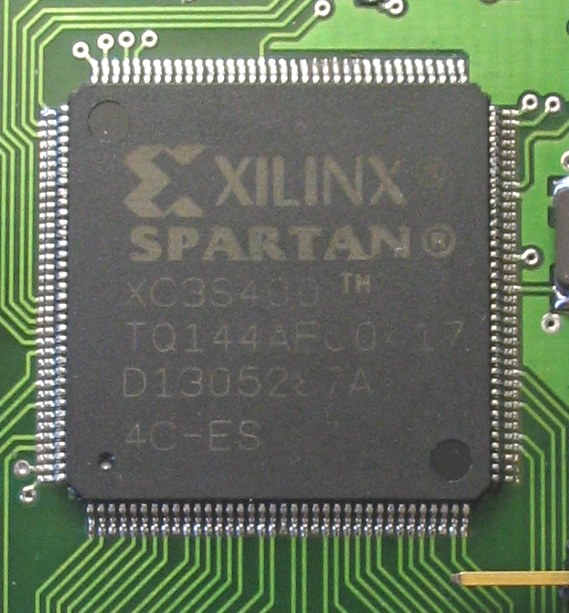
\includegraphics[scale=0.75]{images/fpga}
    }
\end{frame}

\note[itemize] {
    \item Il s’agit d’un réseau logique programmable. À l’aide d’un langage de
        description matériel on va cabler des blocs logiques ensemble. Dans ce
        composants, il y en a 400 000.

    \item Pour vous donner une idée, toujours dans l’idée de faire clignoter une
        led, voici ce que ça donne en verilog.
}

\begin{frame}
    \frametitle{FPGA}

    \addtooverlay<.(1)>{
        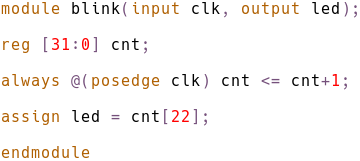
\includegraphics[scale=0.4]{images/sources/verilog}
    }
    \addtooverlay<.(1)>{
        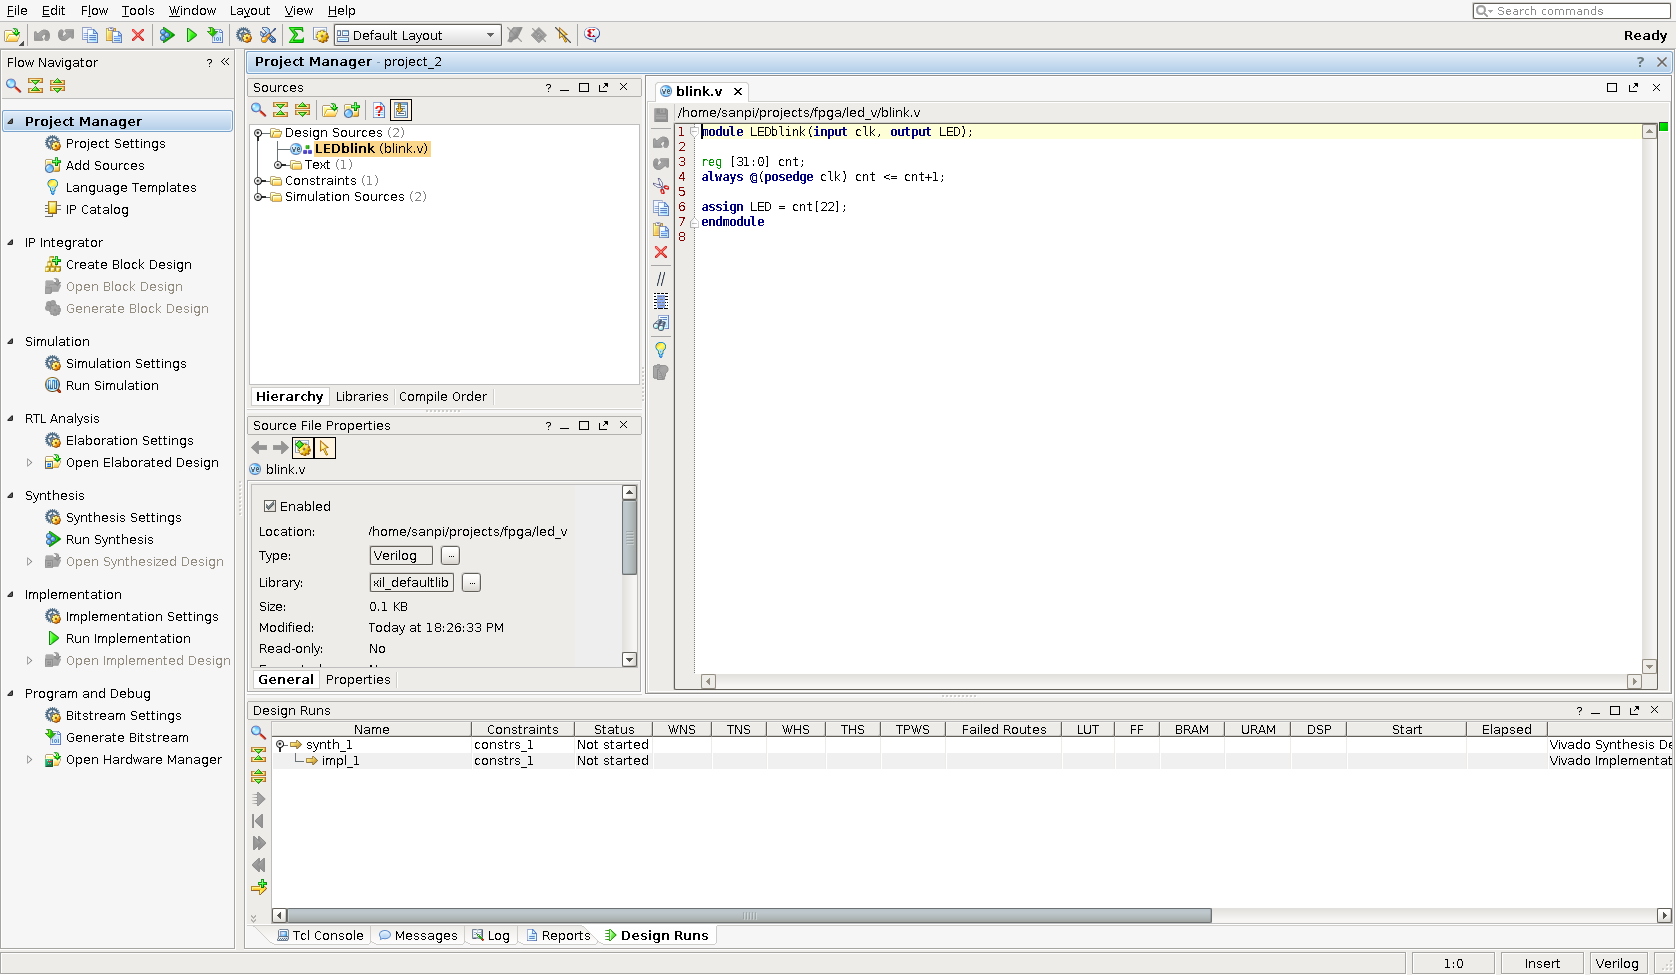
\includegraphics[scale=0.20]{images/xilinx}
    }
\end{frame}

\note[itemize] {
    \item Alors on déclare un module « blink » avec en entrée le signal de
        l’hologe et en sortie un gpio qui va controller notre LED. Un second
        fichier fait la correspondance entre ces noms et les numéros de gpio.

    \item Ensuite on a un registre de 32 bits, nommé « cnt ».

    \item Sur le frond montant du signal de l’horloge, on incrémente ce
        registre.

    \item Enfin, on assigne le 23ième bit de notre registre à notre LED. Donc
        lorsque notre compteur aura ce bit à 1, la led sera allumée.

    \item Alors quand j’ai commencé à m’intéressé au fpga, j’ai eu l’impression
        de revenir à mes débuts en développement.

    \item Il faut télécharger un outils propriétaire de 8Go. J’ai passé quelques
        mois à comprendre comment ça marche pour produire un plugin pour waf (un
        équivalent de make) toujours dans l’idée de retrouver mes outils
        habituels. Et le fabricant a sortie un nouvel outils…

    \item Heureusement, entre temps, Clifford Wolf à publier une chaine de
        synthère entièrement libre.
}

% {{{ Outlis libres
\begin{frame}
    \frametitle{Outils libres}

    \begin{itemize}
        \item yosys
        \item arachne-pnr
        \item icestorm
    \end{itemize}
\end{frame}

\note[itemize] {
    \item Ce qui est bien avec les logiciels libres, c’est qu’il y a toujours
        des gens pour avoir des idées géniales pour les enrichirs.
}
% }}}
% {{{ Icestudio
\begin{frame}
    \frametitle{Icestudio}
\end{frame}

\note[itemize] {
    \item Première idée géniale, icestudio
}

\begin{frame}
    \frametitle{Icestudio}

    \addtooverlay<.(1)>{
        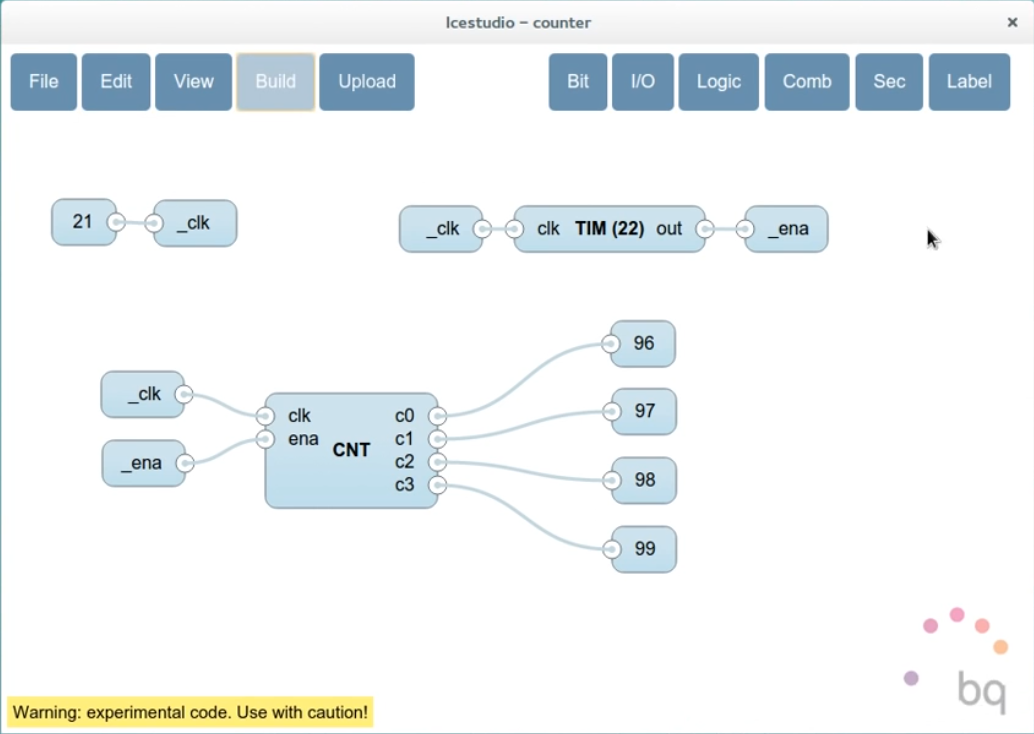
\includegraphics[scale=0.28]{images/icestudio}
    }
\end{frame}

\note[itemize] {
    \item Il s’agit d’un éditeur graphique.
}
% }}}
% {{{ Ecowlogic
\begin{frame}
    \frametitle{Ecowlogic}

    \addtooverlay<.(1)>{
        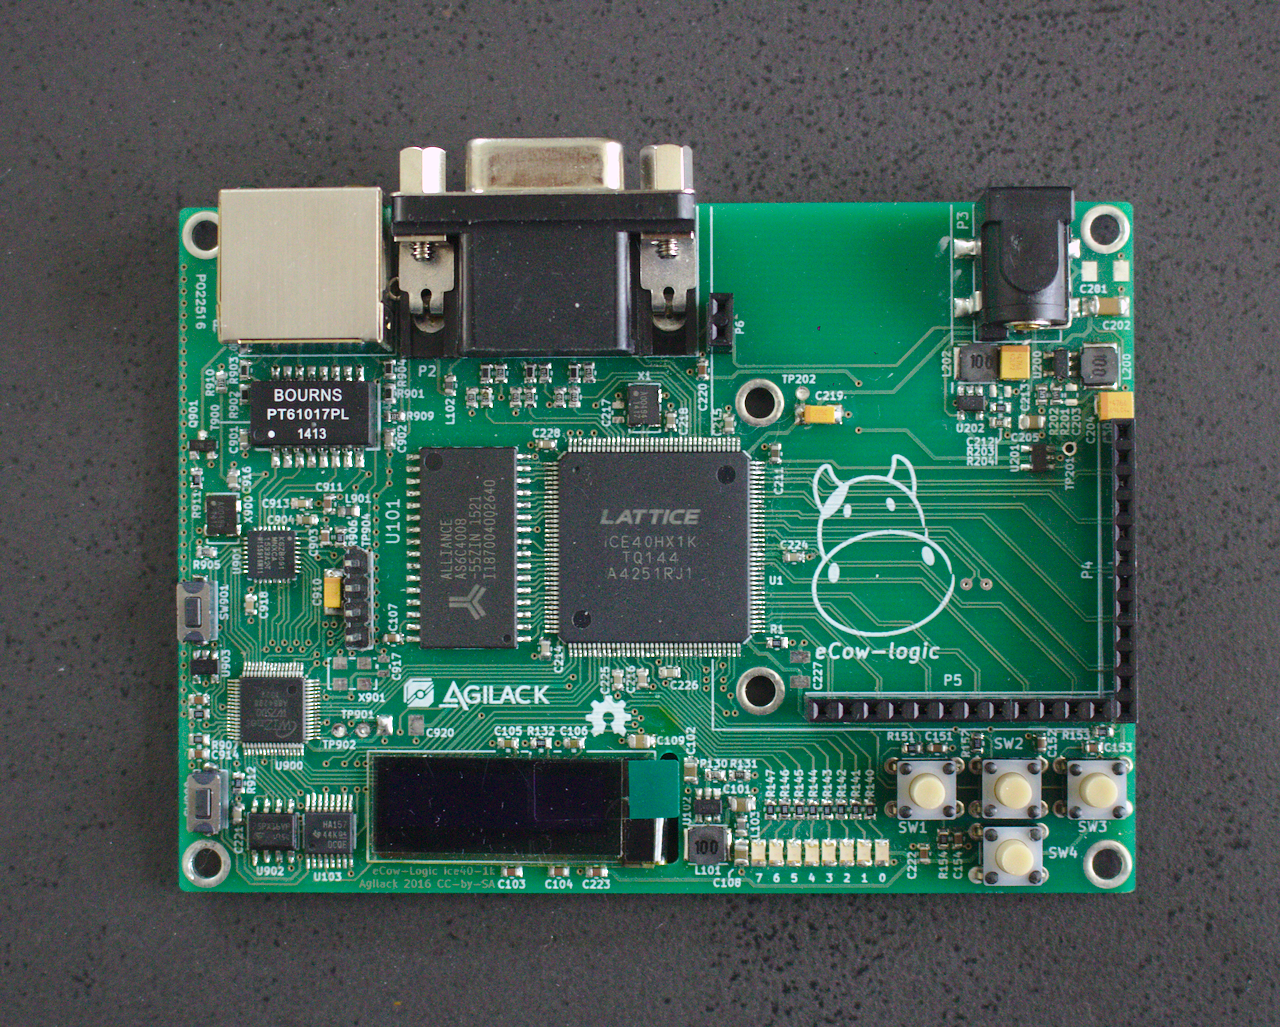
\includegraphics[scale=0.20]{images/ecowlogic/card}
    }
    \addtooverlay<.(1)>{
        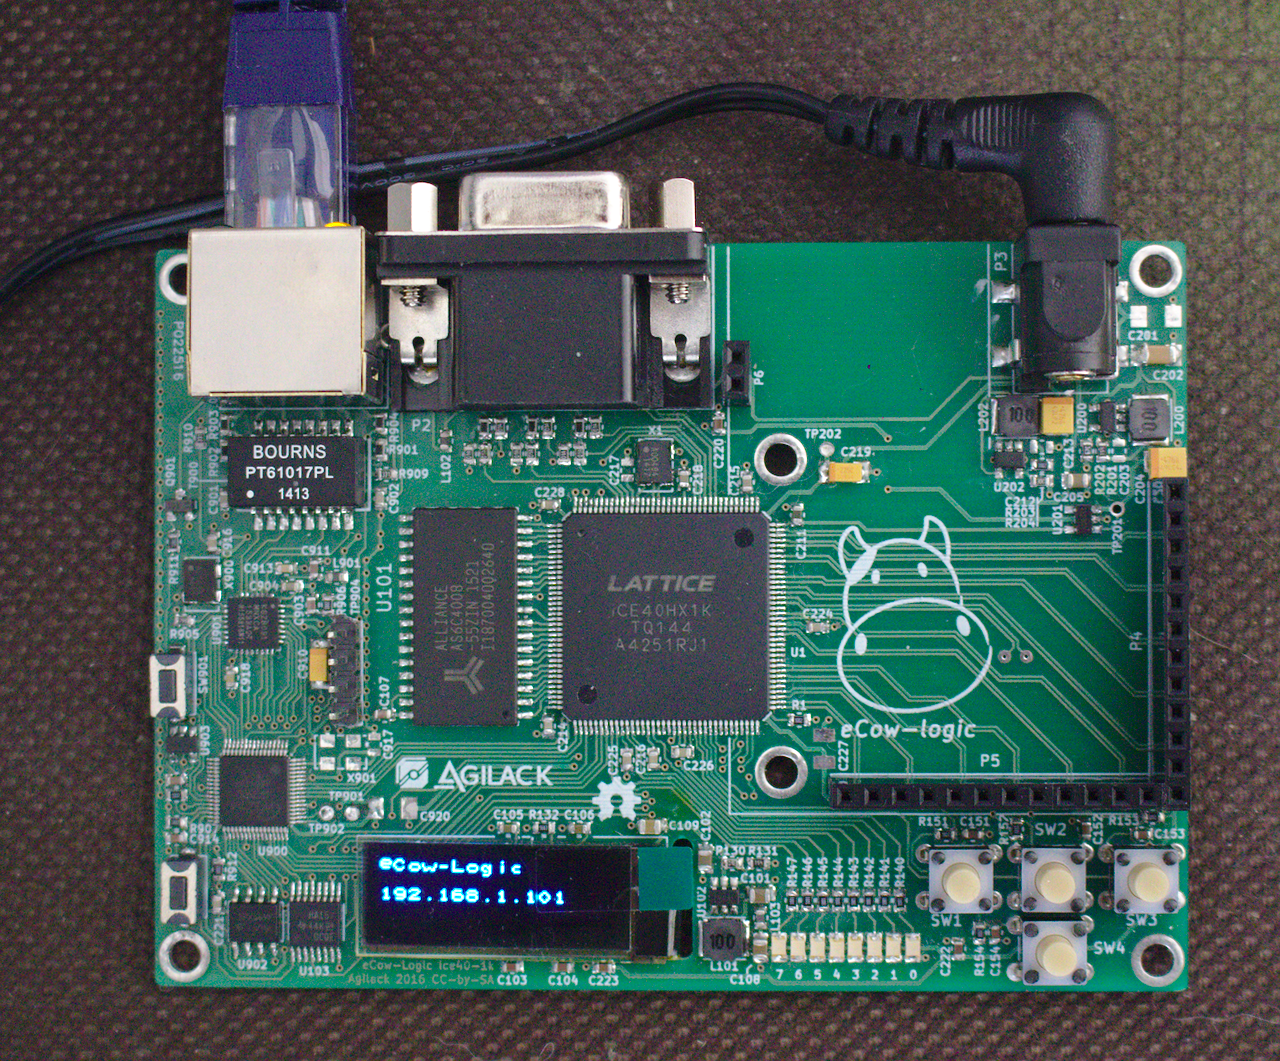
\includegraphics[scale=0.20]{images/ecowlogic/pluged}
    }
    \addtooverlay<.(1)>{
        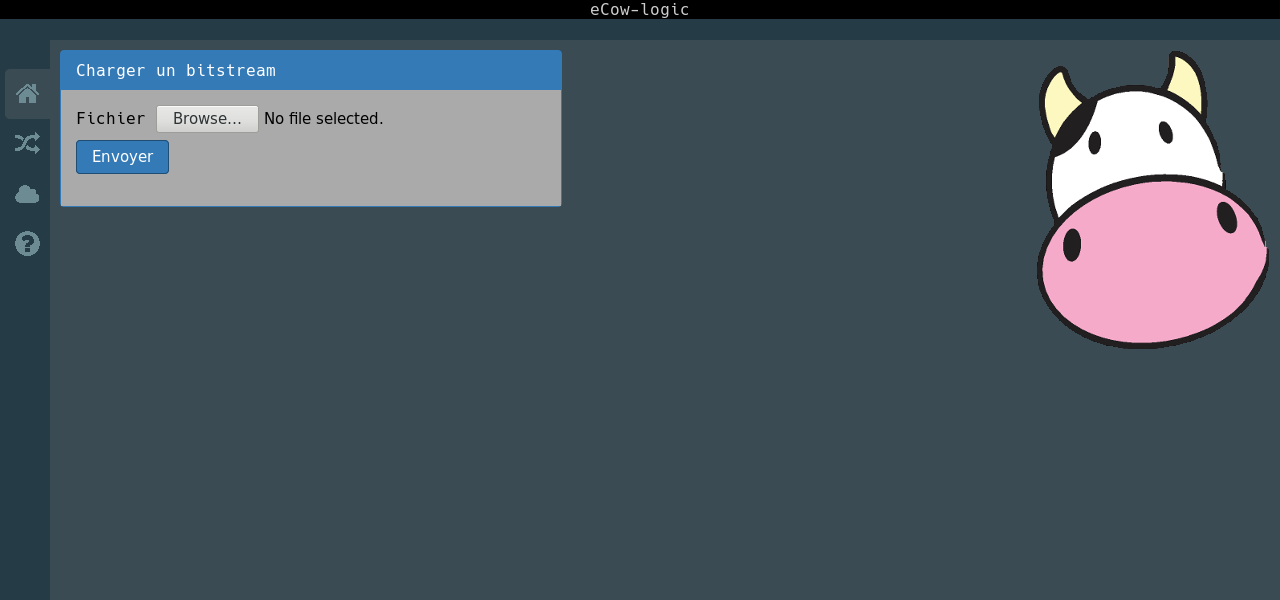
\includegraphics[scale=0.28]{images/ecowlogic/upload}
    }
    \addtooverlay<.(1)>{
        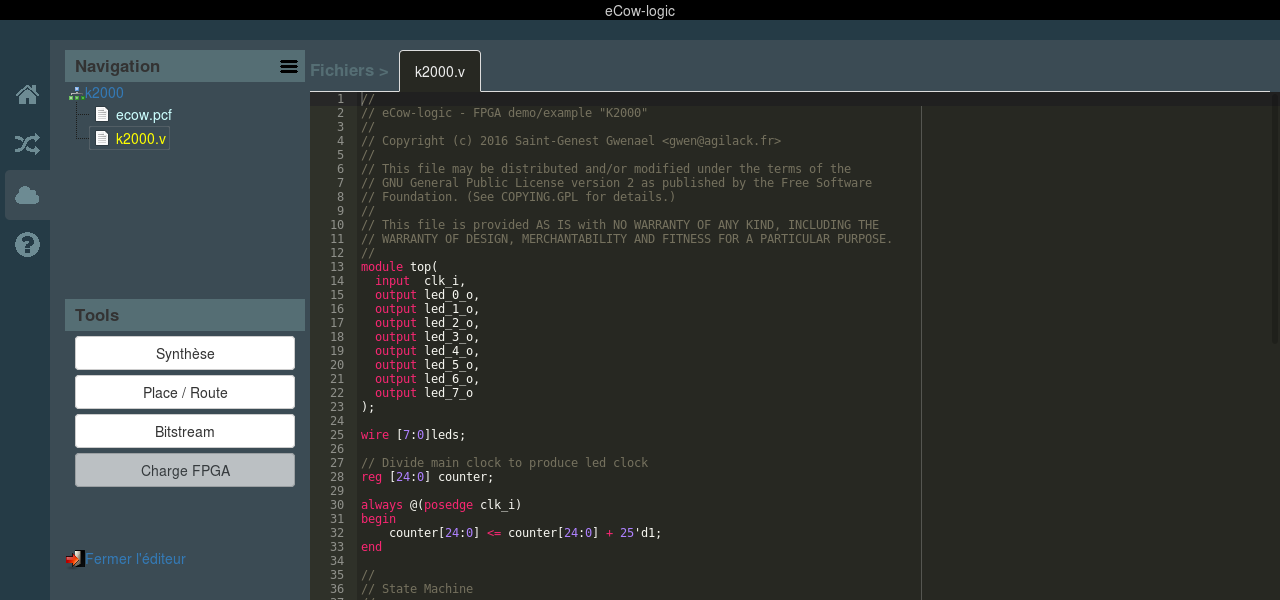
\includegraphics[scale=0.28]{images/ecowlogic/cowlab4}
    }

    \begin{itemize}[<+->]
        \item http POST 192.168.1.114/pld @blink.bin
        \item démo ?
    \end{itemize}
\end{frame}

\note[itemize] {
    \item Second projet, pour lequel je serais moins partial puisque je
        participe au développement va encore plus loin dans la simplicité
        d’installation, si j’osai je parlerai de FPGA as a service.
}
% }}}
% }}}

% {{{ Référence
\section{Références}
\begin{frame}
    \frametitle{Références}

    \begin{itemize}
        \item \small \url{https://media.ccc.de/v/camp2015-6634-pushing_the_limits_of_diy_electronics}
    \end{itemize}

    \begin{itemize}
        \item \small \url{http://oomlout.com/BBAC/src/guide/BBAC-01-guide-OOML-WEB.pdf}
        \item \small \url{http://www.nongnu.org/avr-libc/}
        \item \small \url{https://learn.sparkfun.com/tutorials/installing-an-arduino-bootloader}
        \item \small \url{https://www.arduino.cc/en/Hacking/Bootloader?from=Main.Bootloader}
        \item \small \url{http://dangerousprototypes.com/docs/Bus_Pirate_AVR_Programming}
        \item \small \url{http://www.jtxp.org/tech/tinysafeboot_en.htm}
    \end{itemize}
\end{frame}

\begin{frame}
    \frametitle{Références}

    \begin{itemize}
        \item \small \url{https://fr.wikipedia.org/wiki/Syst\%C3\%A8me_g\%C3\%A9n\%C3\%A9ral_harmonis\%C3\%A9_de_classification_et_d\%27\%C3\%A9tiquetage_des_produits_chimiques}
    \end{itemize}

    \begin{itemize}
        \item \small \url{http://wiki.electrolab.fr/Projets:Lab:2015:SolderStation:Manuel}
        \item \small \url{http://dangerousprototypes.com/blog/2012/06/14/workshop-video-how-to-make-a-simple-soldering-flux/}
        \item \small \url{http://www.instructables.com/id/Heatless-cold-Toner-Transfer-for-PCB-Making/}
    \end{itemize}

    \begin{itemize}
        \item \small \url{https://media.ccc.de/v/eh16-40-verilog_synthesis_and_more_with_yosys}
        \item \small \url{http://www.clifford.at/yosys/}
        \item \small \url{http://www.clifford.at/icestorm/}
        \item \small \url{https://github.com/bqlabs/icestudio}
        \item \small \url{http://ecowlogic.fr/}
    \end{itemize}
\end{frame}
% }}}

% {{{ Questions
\begin{frame}
    \frametitle{Questions ?}

    \begin{figure}
        
\includegraphics{images/qrcode}
        \captionsetup{labelformat=empty}
        \caption{
            \tiny{
                \url{https://github.com/sanpii/slides/releases/download/pses2016/push-limit-electronic.pdf}
            }
        }
    \end{figure}
\end{frame}
% }}}
\end{document}
